\documentclass[5p,times]{elsarticle}

\usepackage[utf8]{inputenc}
\usepackage[T1]{fontenc}
\usepackage{amsmath}
\usepackage{amssymb}
\usepackage{amsthm}
\usepackage{mathtools}
\usepackage{booktabs}
\usepackage{graphicx}
\usepackage{xcolor}
\usepackage{colortbl}
\usepackage{listings}
\usepackage{hyperref}
\usepackage{multirow}
\usepackage{array}
\usepackage{float}
\usepackage{pifont}
\usepackage{algorithm}
\usepackage{algorithmic}
\usepackage{tikz}
\usepackage{pgfplots}
\pgfplotsset{compat=1.18}
\usepackage{subcaption}

\usetikzlibrary{arrows.meta,positioning,shapes.geometric,fit,calc,decorations.pathmorphing}

\graphicspath{{figures/}}


\hbadness=10000
\vbadness=10000
\hfuzz=100pt
\vfuzz=100pt
\emergencystretch=3em

\makeatletter
\DeclareFontShape{T1}{txr}{m}{scit}{<->ssub*txr/m/sc}{}
\pdfstringdefDisableCommands{%
  \def\corref#1{}%
  \def\cnotenum#1{}%
  \def\@corref#1{}%
}
\makeatother

\renewcommand{\algorithmicrequire}{\textbf{Input:}}
\renewcommand{\algorithmicensure}{\textbf{Output:}}

\newtheorem{definition}{Definition}[section]
\newtheorem{property}{Property}[section]
\newtheorem{proposition}{Proposition}[section]

\lstset{
  basicstyle=\ttfamily\small,
  breaklines=true,
  commentstyle=\itshape\color{gray},
  keywordstyle=\bfseries\color{blue},
  stringstyle=\color{red},
  showstringspaces=false,
  frame=single,
  backgroundcolor=\color{white!95!gray}
}

\journal{Ad Hoc Networks}

\begin{document}

\begin{frontmatter}

\title{MAPPO-Based Routing with Adaptive 3D Broadcast Suppression for Flying Ad Hoc Networks}

\author[inst1]{Sabri Allani\corref{cor1}}
\cortext[cor1]{Corresponding author}
\ead{sabri.allani@ensi-uma.tn}
\address[inst1]{ENSI, University of Manouba, Manouba 2010, Tunisia}

\begin{abstract}
\sloppy
Flying Ad Hoc Networks (FANETs) suffer from rapid topology changes, short link lifetimes, and severe rebroadcast redundancy, which jointly degrade routing reliability and channel efficiency. Existing FANET protocols often optimize forwarding and broadcast control separately, which limits adaptation under dynamic 3D mobility and heterogeneous traffic priorities. This paper presents ASTRO-FANET, a cooperative routing framework based on Multi-Agent Proximal Policy Optimization (MAPPO) under centralized training and decentralized execution. Each UAV selects among forwarding, aggregation, suppression, broadcast, and role-switching actions from local context, while Adaptive 3D Broadcast Storm Mitigation (A3D-BSM) applies thresholded, context-dependent suppression to control rebroadcast redundancy.

The framework is evaluated in CupCarbon simulation with swarm sizes from 10 to 40 UAVs under Gauss--Markov and RPGM mobility, using 30 independent runs per configuration, 95\% confidence intervals, and corrected statistical significance tests. Baselines include AODV, GPSR, OLSR, epidemic flooding, and a DQN-based Q-routing protocol. Metrics include packet delivery ratio, end-to-end delay, throughput, broadcast redundancy, control overhead, and energy per useful bit. In medium-to-dense swarms, ASTRO-FANET achieves 92.8\% packet delivery ratio with 64\,ms end-to-end delay at $N=30$, improving over the best classical baseline by 12.7 percentage points in PDR while reducing broadcast redundancy by 91\% relative to epidemic flooding ($p < 0.001$). Under a high-speed sparse stress scenario ($N=10$, 25--40\,m/s), the advantage narrows to 2.1\,pp over epidemic flooding with higher control overhead, indicating an explicit operating boundary. Ablation and sensitivity analyses support the contribution of cooperative MARL decisions, adaptive suppression, and representation design, including a same-dimensional MLP autoencoder control. The security layer is integrated as a routing-support module with preliminary selective-dropping Byzantine evaluation; comprehensive adversarial benchmarking is left for future work.
\fussy
\end{abstract}

\begin{keyword}
FANET \sep UAV Routing \sep Multi-Agent Reinforcement Learning \sep Broadcast Storm Mitigation \sep Throughput Optimization \sep Ad Hoc Networks
\end{keyword}

\end{frontmatter}

\section{Introduction}
\label{sec:introduction}

Flying Ad Hoc Networks (FANETs) connect cooperative UAVs without fixed infrastructure and support applications such as emergency mapping, environmental monitoring, and temporary connectivity restoration~\cite{bekmezci2013fanets,khan2020routing,lakew2020routing,motlagh2016uaviot,gharibi2016iod}. Compared with MANETs and VANETs, FANETs operate under faster topology dynamics, shorter link duration, and stronger coupling between communication and mission execution.

These characteristics directly impact routing and dissemination. In particular, rebroadcast-heavy operation causes severe channel contention in 3D spaces, while strict delay constraints for high-priority traffic limit the use of static suppression rules. At the same time, purely reactive or purely geographic forwarding can underperform when link quality, mobility, queue pressure, and residual energy change simultaneously. Therefore, FANET routing requires online policies that jointly optimize delivery, latency, overhead, and energy rather than tuning each objective independently.

Despite sustained progress in FANET routing, three practical gaps remain for highly dynamic 3D swarms: (i) routing and broadcast suppression are often treated separately, (ii) adaptive policies are commonly trained on fixed feature vectors that may under-represent heterogeneous local context, and (iii) security-aware coordination is frequently added as an overlay rather than incorporated into the routing decision loop. This paper focuses on the first two gaps as the primary validated contribution, and treats security integration as a support layer with preliminary assessment.

\begin{figure}[t]
\centering
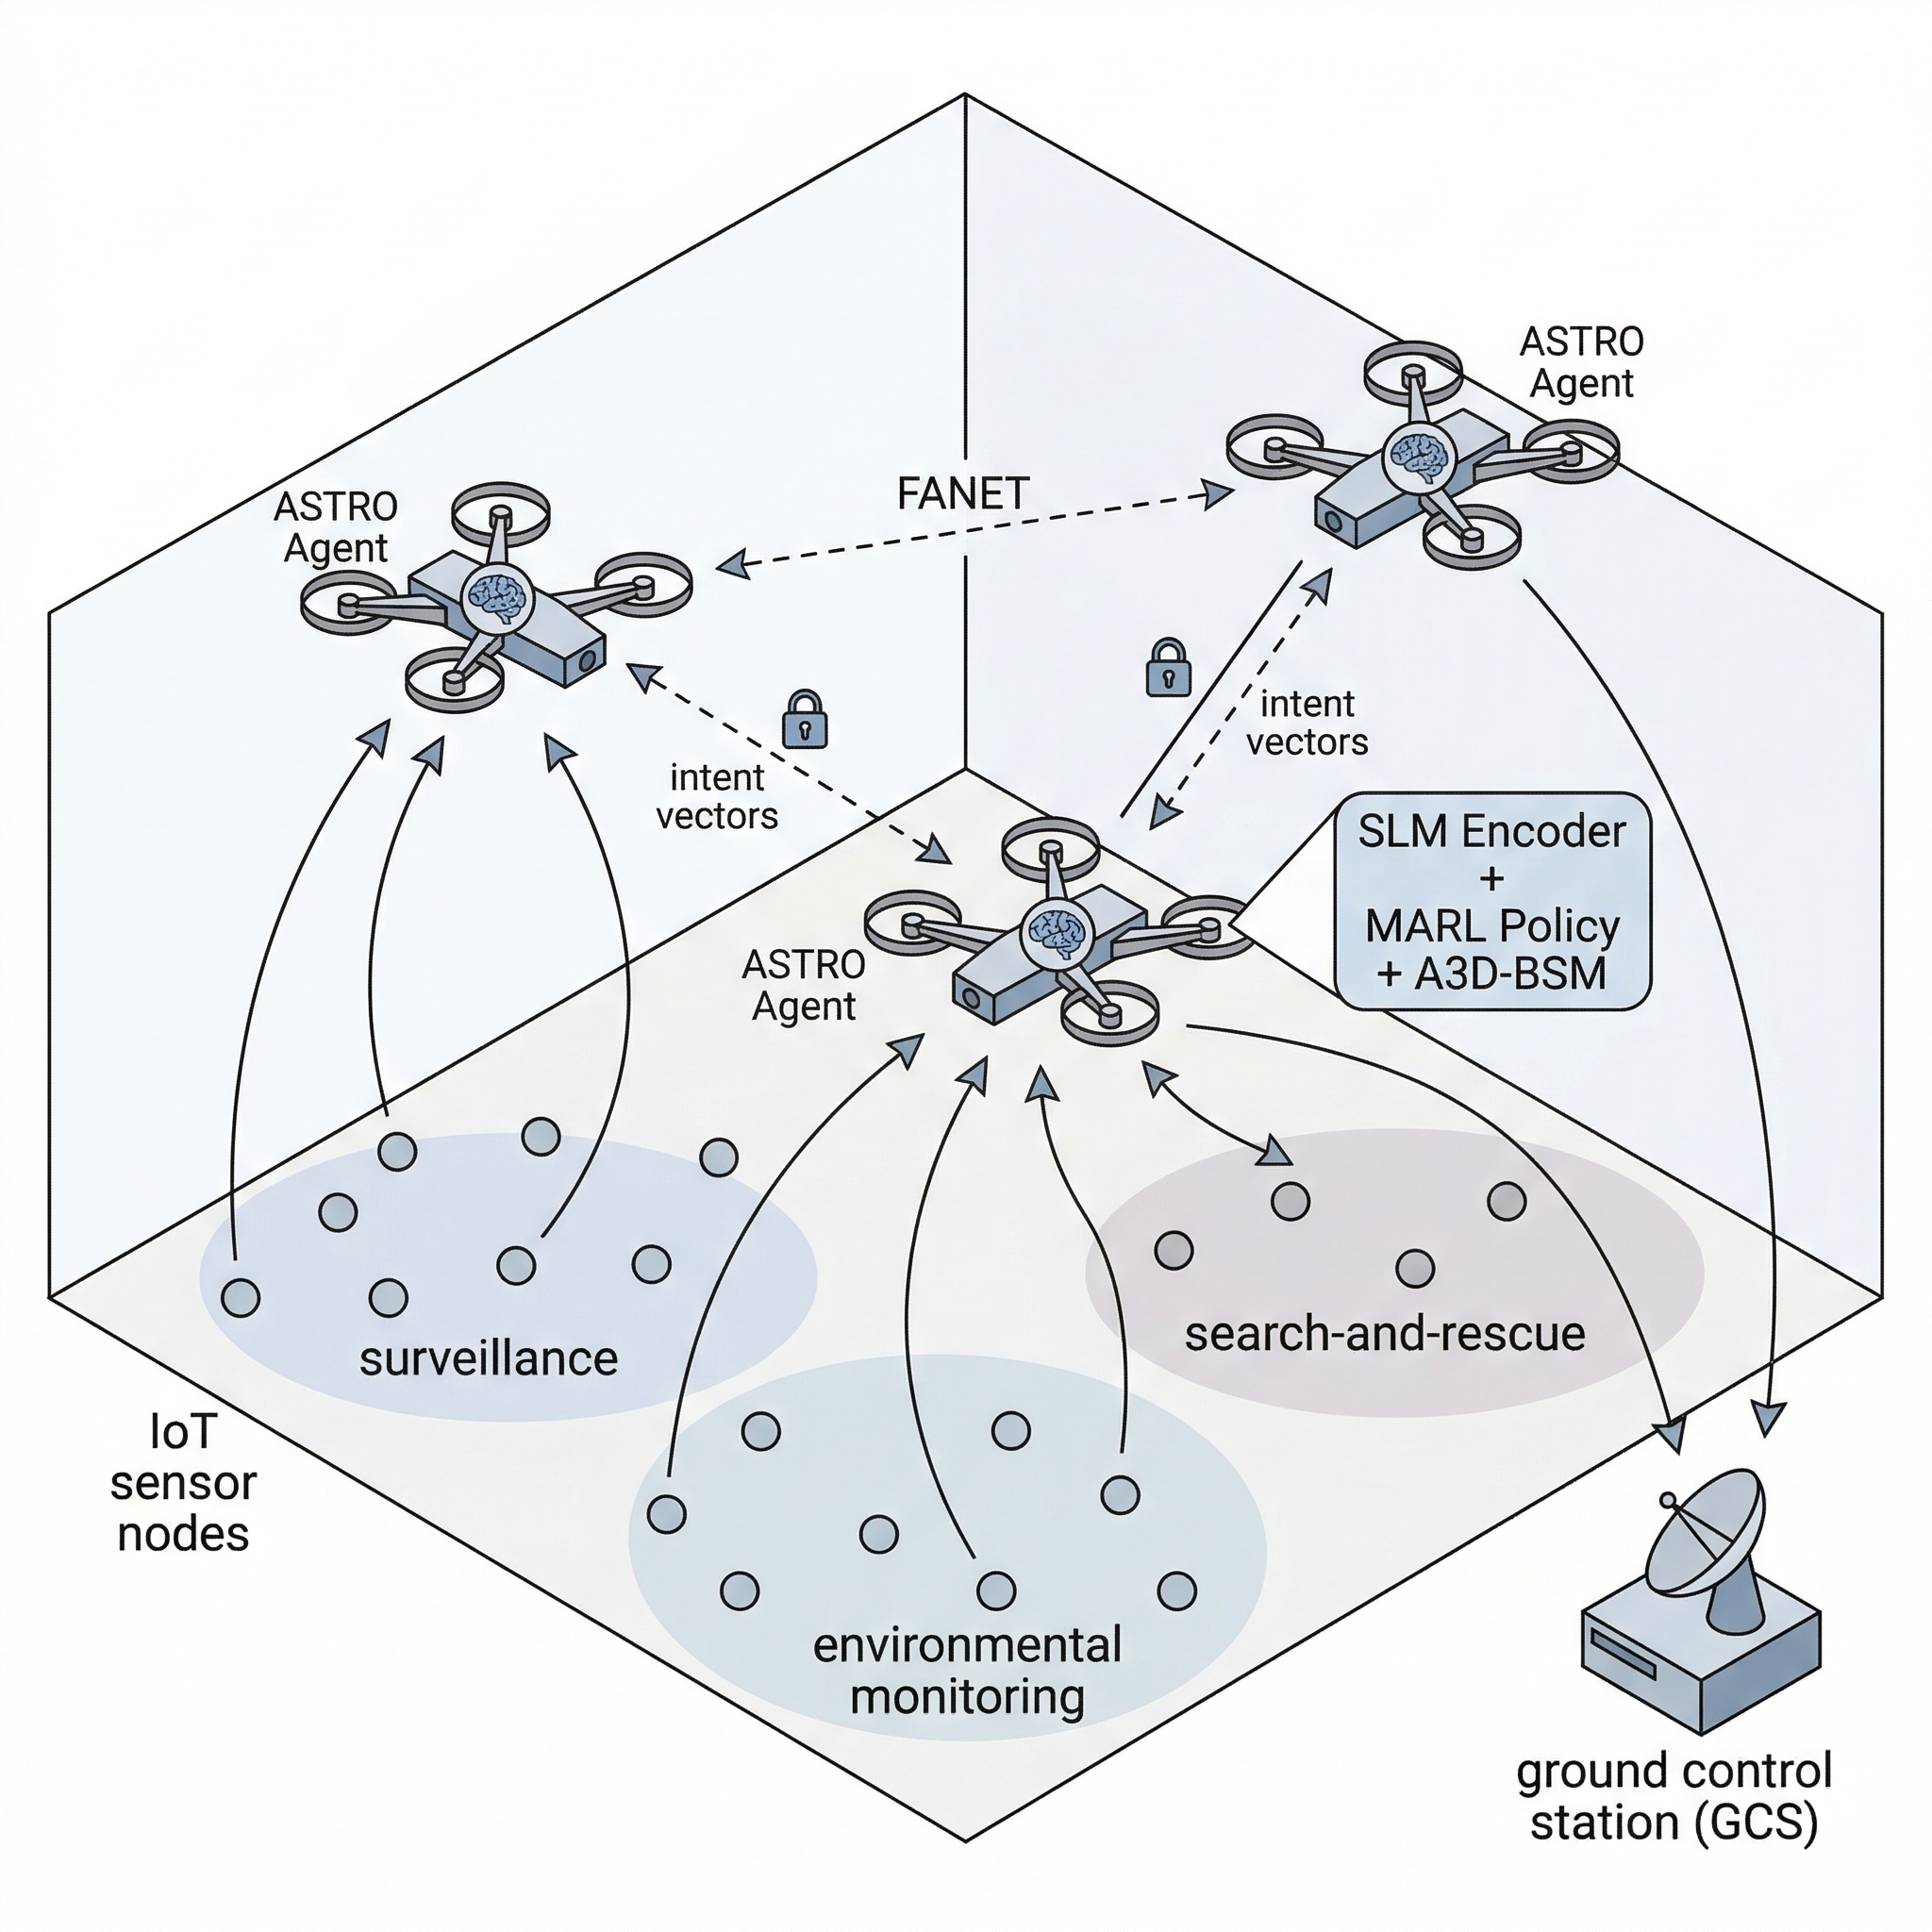
\includegraphics[width=\linewidth]{figure1.png}
\caption{Overview of ASTRO-FANET: local state encoding, cooperative policy-based routing, and adaptive broadcast suppression in a 3D FANET.}
\label{fig:fanet-overview}
\end{figure}

\subsection{Problem statement and scope}

We address distributed routing in a multi-UAV FANET with heterogeneous traffic classes and dynamic neighborhood changes. The target problem is to maximize reliable packet delivery while controlling delay, throughput efficiency, control overhead, and communication energy under fast 3D mobility. The validated scope of this paper is simulation-based evaluation of joint routing, aggregation, and adaptive broadcast control (Layers~1--3), together with preliminary assessment of the security-support mechanism under a selective-dropping Byzantine model. Real-flight validation, large-scale deployment beyond the studied swarm range, and comprehensive adversarial benchmarking are outside the present scope.

\subsection{Contributions}

This work makes the following technical contributions:

\begin{enumerate}
\item \textbf{Cooperative MARL routing formulation.} We formulate FANET routing as a decentralized partially observable Markov game with explicit state, action, and reward definitions, and train policies with MAPPO under centralized training and decentralized execution.

\item \textbf{Joint forwarding--suppression decision design.} We define a unified routing action space and integrate A3D-BSM through an explicit thresholded decision rule with adaptive 3D suppression-zone parameterization.

\item \textbf{Context representation study under simulation constraints.} We incorporate SLM-based state encoding in the decision pipeline and evaluate its contribution against fixed features and a same-dimensional MLP autoencoder baseline, while explicitly modeling SLM embeddings through pre-computation and interpolation in simulation.

\item \textbf{Reproducible simulation campaign with bounded claims.} We provide a CupCarbon-based evaluation with explicit scenario parameters, 30 independent runs per setting, 95\% confidence intervals, and corrected statistical tests against AODV, GPSR, OLSR, epidemic flooding, and a DQN-based Q-routing baseline, including stress-scenario analysis to delineate the method's operating regime.

\item \textbf{Security-support integration with preliminary assessment.} We specify authenticated intent exchange and trust scoring within the routing loop, and report preliminary selective-dropping Byzantine results without claiming comprehensive adversarial robustness.
\end{enumerate}

\subsection{Paper organization}

Section~\ref{sec:related} critically reviews prior FANET routing, broadcast suppression, learning-based routing, and security-aware designs, then identifies the targeted gap. Section~\ref{sec:framework} presents the system model and the proposed routing methodology. Section~\ref{sec:experiments} reports simulation settings and results. Section~\ref{sec:discussion} analyzes robustness and validity threats. Section~\ref{sec:conclusion} concludes the paper.

\section{Related Work and Research Gap}
\label{sec:related}

This section reviews prior work along four axes that are directly relevant to the target problem: FANET routing protocols, broadcast suppression, learning-based routing, and security-aware coordination. The focus is on methodological limitations that affect routing performance under fast 3D mobility.

\subsection{FANET routing, topology, and data dissemination}

Classical FANET routing protocols are generally adapted from reactive, proactive, and geographic MANET/VANET families~\cite{bekmezci2013fanets,khan2020routing,lakew2020routing,oubbati2019routing}. Their core limitation is not conceptual correctness but adaptation speed. Reactive protocols incur rediscovery delays after link breakage; proactive protocols trade stability for high control traffic; geographic approaches rely on neighbor geometry that can become unstable under fast altitude and direction changes. Recent topology-control and clustering methods improve scalability~\cite{alam2022topology,salam2023cluster,nguyen2024adaptive}, but they still depend on fixed heuristics and may underperform when mobility, queue state, and link quality co-vary over short timescales.

\subsection{Broadcast storm problem in ad hoc networks}

The broadcast storm problem is well established in ad hoc networks~\cite{tseng2002broadcast}. Existing mitigation methods (probabilistic timers, counter-based forwarding, and zone-restricted dissemination) reduce redundancy but are typically derived for 2D mobility and homogeneous traffic assumptions. In FANETs, 3D coverage geometry, faster neighborhood turnover, and traffic-priority constraints make static suppression rules less reliable. This motivates adaptive suppression policies that couple channel load, packet urgency, and local topology state.

\subsection{Reinforcement learning for UAV networking}

RL and MARL are increasingly used in UAV networking for relay selection, trajectory control, and resource management~\cite{liu2019rl_routing,lowe2017maddpg,yu2022mappo,zhao2024marl_uav,wang2023drl_fanet}. These studies demonstrate the benefit of adaptive policies, but most optimize a limited objective set (typically throughput or energy) and do not jointly treat routing and broadcast suppression. In addition, many implementations rely on fixed-size engineered state vectors, which can limit representation of heterogeneous context (mobility trends, queue classes, and neighbor reliability) in dense dynamic swarms.

\subsection{Representation learning for networking state encoding}

Recent networking studies report that learned representations can outperform purely hand-crafted features in dynamic decision tasks~\cite{he2024large_networking,mittal2024survey_edge_llm}. Small language models and compact transformer encoders are particularly attractive for edge settings because they can encode variable-length contextual input after quantization~\cite{abdin2024phi3,zhang2024tinyllama,lin2024awq,xu2024survey_slm}. In this paper, SLM-based encoding is evaluated as one representation option for routing state compression rather than as an autonomous reasoning layer.

\subsection{Security in UAV ad hoc networks}

Security is a critical concern in FANETs due to open wireless channels, physical exposure, and decentralized control~\cite{chriki2019fanet_security,khan2020uav_security,singh2023survey_fanet_security}. Existing schemes typically treat trust and authentication as external overlays to routing decisions. In ASTRO-FANET, the security layer is integrated as a routing-support module (authenticated control exchange plus behavior scoring), with preliminary selective-dropping evaluation and without a full adversarial benchmark campaign.

\subsection{Research gap and positioning}

Table~\ref{tab:related} synthesizes the positioning of ASTRO-FANET relative to existing literature across six critical dimensions.

\begin{table*}[t]
\centering
\caption{Comparative positioning of ASTRO-FANET with respect to the main literature streams.}
\label{tab:related}
\scriptsize
\begin{tabular}{p{2.4cm}p{1.5cm}p{1.5cm}p{1.5cm}p{1.5cm}p{1.5cm}p{3.5cm}}
\toprule
Reference & FANET routing & Broadcast storm & RL/MARL & SLM/LLM & Security & Key limitation \\
\midrule
\cite{bekmezci2013fanets,khan2020routing} & \ding{51} & \ding{55} & \ding{55} & \ding{55} & \ding{55} & Survey/taxonomy, no adaptive control \\
\cite{oubbati2019routing,lakew2020routing} & \ding{51} & Partial & \ding{55} & \ding{55} & \ding{55} & Heuristic-based, not learning-driven \\
\cite{allani2018dpms} & VANET & \ding{51} & \ding{55} & \ding{55} & \ding{55} & 2D only, static ZOR via FCA \\
\cite{tseng2002broadcast} & MANET & \ding{51} & \ding{55} & \ding{55} & \ding{55} & Ground networks, rule-based suppression \\
\cite{liu2019rl_routing,wang2023drl_fanet} & \ding{51} & \ding{55} & Single & \ding{55} & \ding{55} & No multi-agent cooperation \\
\cite{zhao2024marl_uav} & Partial & \ding{55} & \ding{51} & \ding{55} & \ding{55} & Trajectory focus, not broadcast \\
\cite{maatouk2024llm_telecom,bariah2024llm_network} & \ding{55} & \ding{55} & \ding{55} & LLM & \ding{55} & Infrastructure-side, not on-board UAV \\
\cite{chriki2019fanet_security,khan2020uav_security} & Partial & \ding{55} & \ding{55} & \ding{55} & \ding{51} & Add-on security, not jointly optimized with routing \\
\textbf{ASTRO-FANET} & \ding{51} & \ding{51} & \ding{51} & SLM$^\dagger$ & \ding{51} & \textbf{Proposed in this paper} \\
\bottomrule
\multicolumn{7}{l}{\scriptsize $^\dagger$SLM encoder emulated via $k$-NN interpolation over pre-computed Phi-3-mini embeddings in simulation; see Section~\ref{subsubsec:slm_emulation}.}
\end{tabular}
\end{table*}

Based on this analysis, four gaps motivate the present paper:

\begin{enumerate}
\item Joint optimization of routing and broadcast suppression remains limited in existing FANET protocols.
\item Learning-based FANET studies rarely integrate multi-objective routing decisions with explicit suppression control.
\item Flexible context encoding for variable-size local observations is under-explored in FANET routing.
\item Security-aware coordination is often specified separately from routing policies and is not systematically evaluated in the same framework.
\end{enumerate}

ASTRO-FANET is designed to address these gaps through cooperative MARL routing with adaptive 3D suppression and contextual state encoding. The next section details the proposed methodology.

\section{Proposed Routing Methodology}
\label{sec:framework}

This section presents the ASTRO-FANET routing methodology. We first define the system model and assumptions, then detail: (i) state encoding, (ii) MAPPO-based routing policy, (iii) adaptive 3D broadcast suppression, and (iv) optional security-support signaling. We then describe the distributed decision cycle and complexity.

\textit{Validation scope.} The routing, aggregation, and broadcast suppression components (Layers~1--3) are fully evaluated through the CupCarbon simulation campaign described in Section~\ref{sec:experiments}. The security layer (Layer~4) is formally specified and assessed through a preliminary selective-dropping Byzantine scenario; comprehensive adversarial benchmarking remains outside the current scope.

\subsection{System model and assumptions}
\label{subsec:system_model}

We consider a FANET composed of $N$ UAVs denoted $\mathcal{U} = \{u_1, u_2, \dots, u_N\}$ operating over a three-dimensional mission area $\mathcal{A} \subset \mathbb{R}^3$. The network is modeled as a time-varying graph $G(t) = (\mathcal{U}, \mathcal{E}(t))$, where an edge $(u_i, u_j) \in \mathcal{E}(t)$ exists if and only if the 3D Euclidean distance $d_{ij}(t) \leq R_{\max}$ and the link quality $q_{ij}(t) \geq q_{\min}$, with $R_{\max}$ denoting the maximum communication range and $q_{\min}$ a minimum signal-to-noise ratio threshold.

Each UAV $u_i$ at time $t$ is characterized by a state vector:
\begin{equation}
\label{eq:uav_state}
\mathbf{s}_i(t) = \big[\mathbf{p}_i(t),\; \mathbf{v}_i(t),\; e_i(t),\; \mathcal{N}_i(t),\; \mathbf{Q}_i(t),\; \mathbf{L}_i(t),\; m_i(t)\big],
\end{equation}
where $\mathbf{p}_i(t) \in \mathbb{R}^3$ is the 3D position, $\mathbf{v}_i(t) \in \mathbb{R}^3$ is the velocity vector, $e_i(t) \in [0,1]$ is the normalized residual energy, $\mathcal{N}_i(t)$ is the current neighbor set, $\mathbf{Q}_i(t)$ is the packet queue descriptor (lengths per priority class), $\mathbf{L}_i(t)$ is the link quality vector to all neighbors, and $m_i(t)$ is the current mission-role indicator (sensing, relaying, aggregating, or gateway).

Packets belong to one of four traffic classes $\mathcal{C} = \{$\textsc{Emergency}, \textsc{Command}, \textsc{Sensing}, \textsc{Telemetry}$\}$, each with a priority level $P_c$ and a maximum tolerable delay $\tau_c^{\max}$. We use $P_c$ (rather than $\pi_c$) for priority to avoid notational conflict with the policy $\pi_{\psi_i}$.

We assume the following: (A1)~each UAV has access to its own GPS coordinates (or an equivalent localization mechanism); (A2)~neighbor discovery and link quality estimation are available through periodic beaconing; (A3)~the SLM is pre-loaded onto each UAV before mission start; (A4)~the MARL policy is trained offline in simulation and deployed as frozen weights; (A5)~at most a fraction $f_{\mathrm{byz}} < 1/3$ of UAVs may be compromised during a mission.

\begin{definition}[ASTRO Agent]
\label{def:astro_agent}
An ASTRO Agent is an autonomous entity running on UAV $u_i$ that perceives its local state $\mathbf{s}_i(t)$, encodes it into a semantic embedding $\mathbf{z}_i(t)$ via the SLM encoder, selects a routing action $a_i(t)$ via the MARL policy, authenticates and shares a compressed intent vector $\boldsymbol{\iota}_i(t)$ with its neighbors, and monitors neighbor behavior for anomalies.
\end{definition}

\begin{figure}[t]
\centering
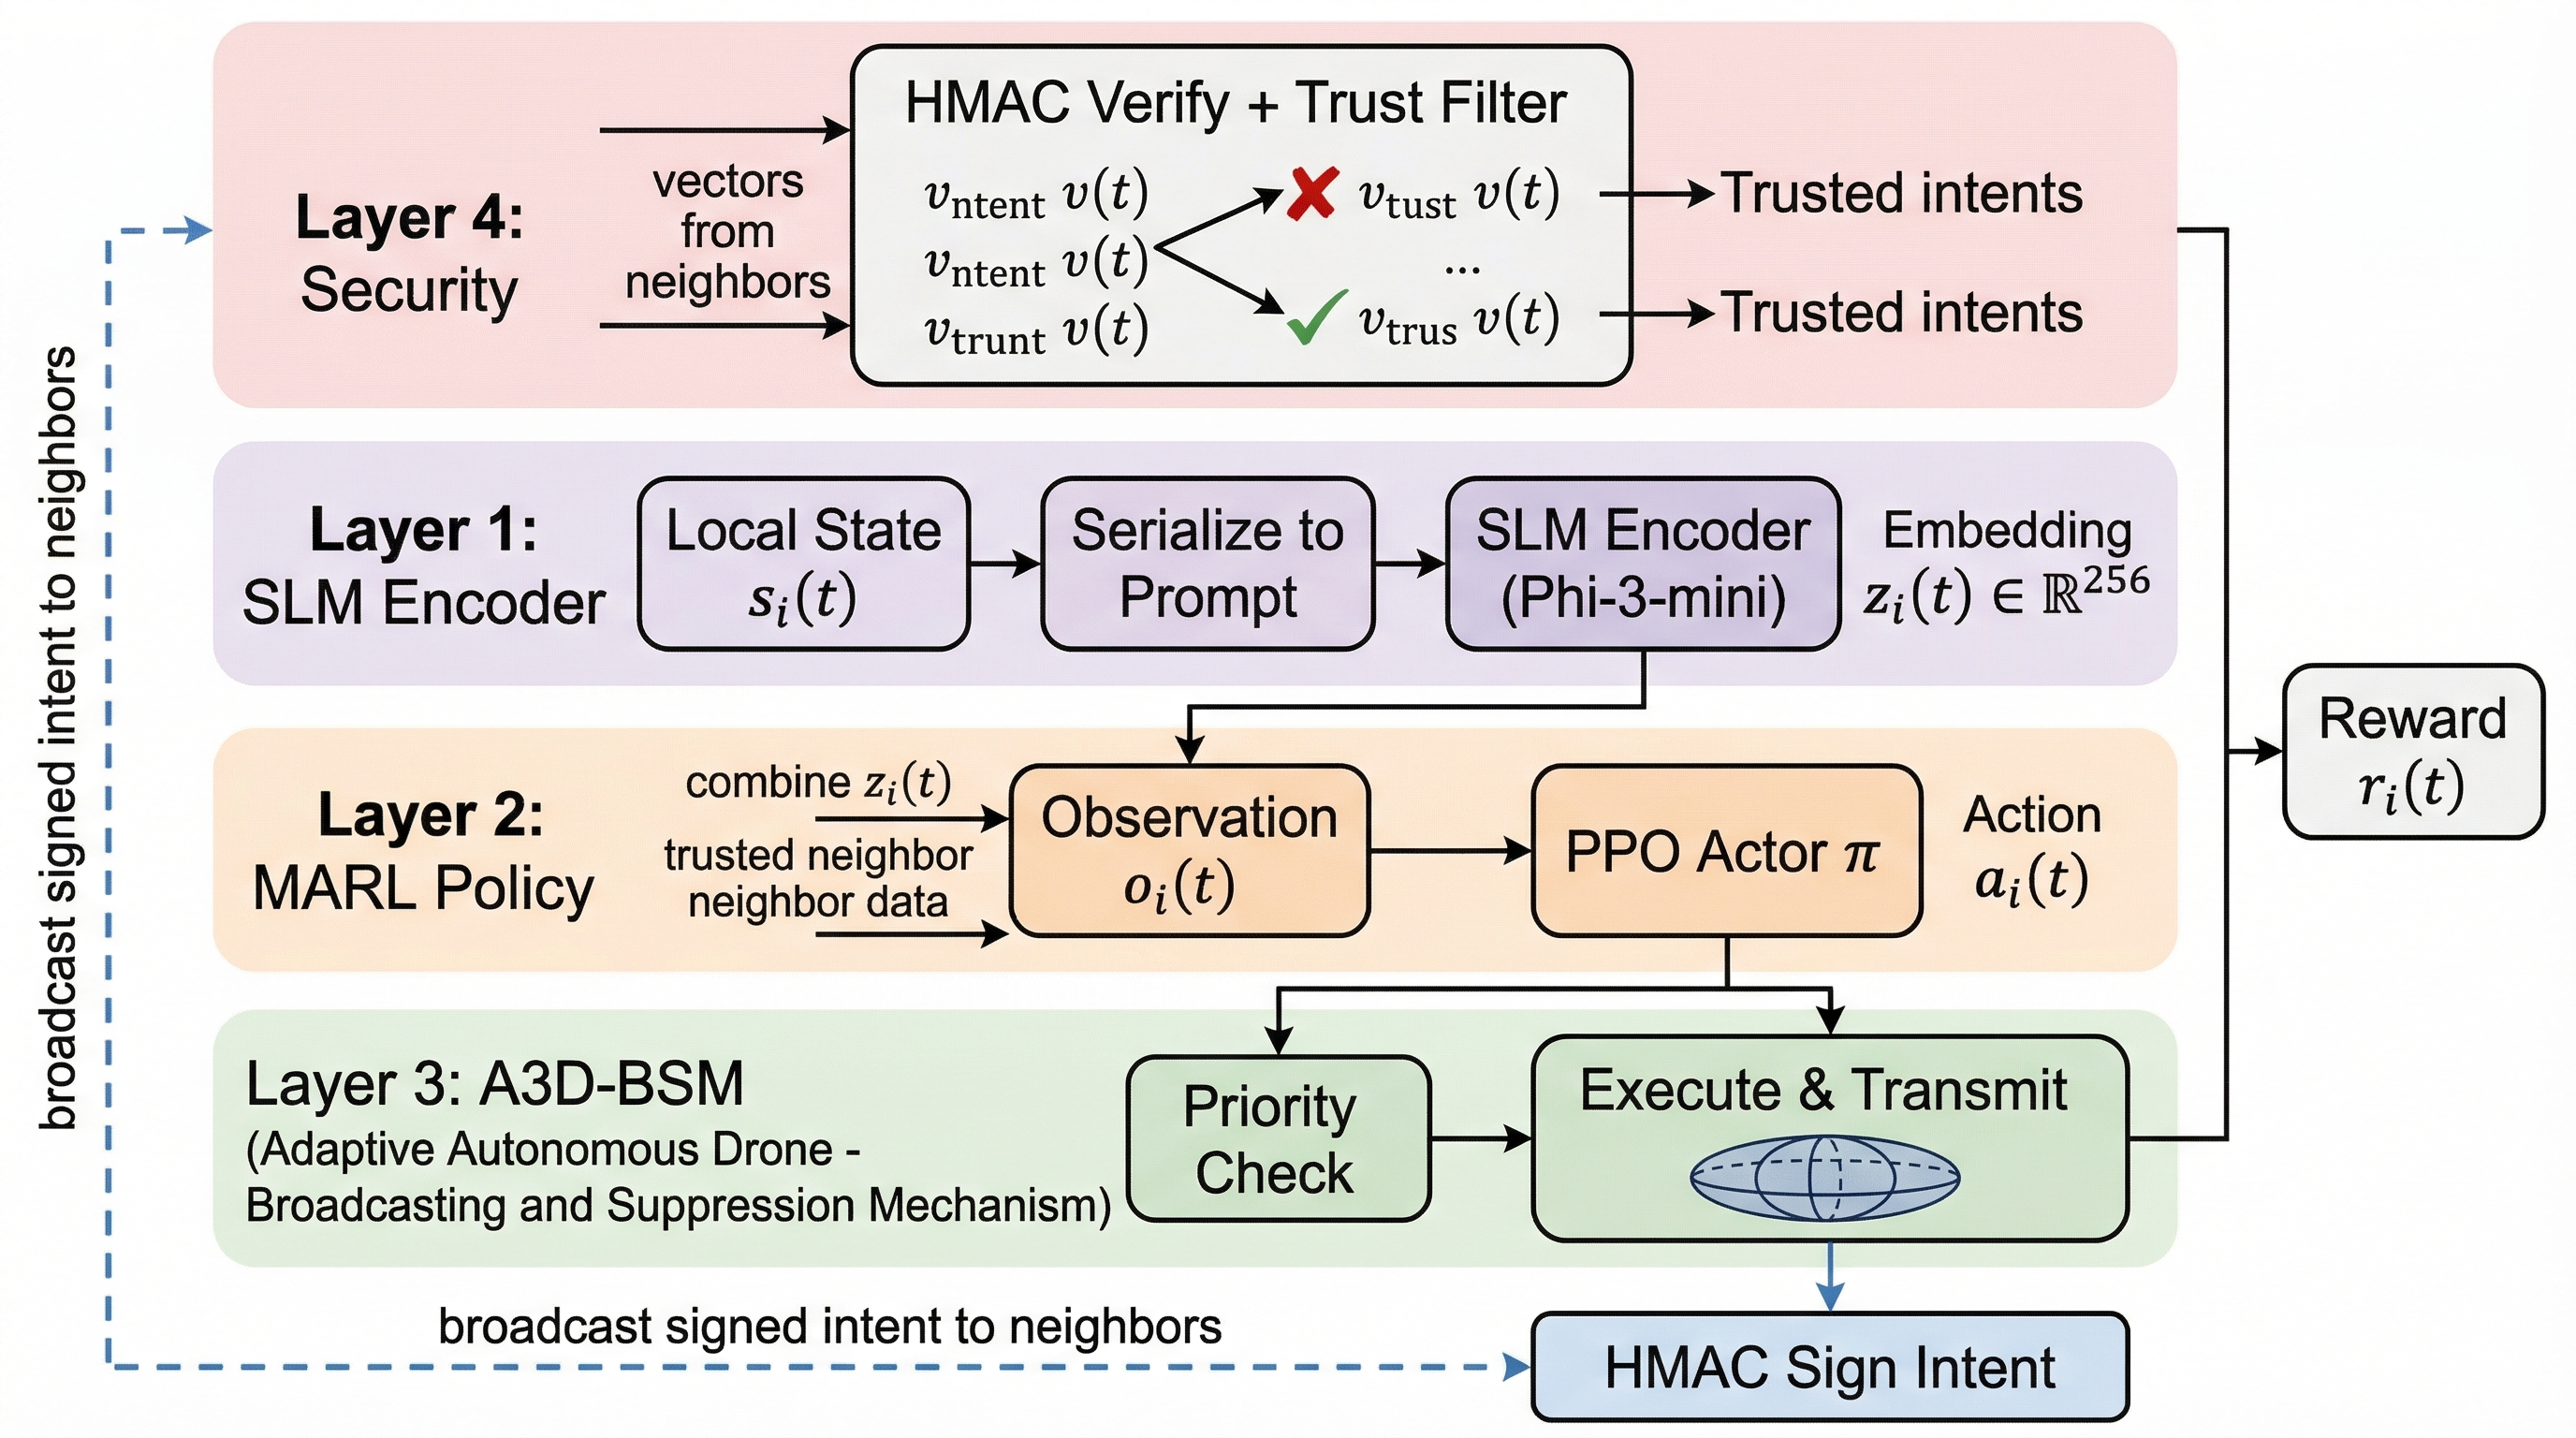
\includegraphics[width=\linewidth]{figure2.png}
\caption{Four-layer architecture of an ASTRO-FANET agent: SLM-based context encoding (Layer~1), MARL policy decision (Layer~2), A3D-BSM broadcast control (Layer~3), and secure resilient communication (Layer~4).}
\label{fig:fanet-pipeline}
\end{figure}

\subsection{Layer 1: SLM-based Semantic Context Encoder}
\label{subsec:slm_encoder}

The first component of ASTRO-FANET uses a quantized Small Language Model as a \emph{perception engine} that transforms heterogeneous, multi-dimensional network state into a compact semantic embedding suitable for reinforcement learning.
This semantic encoding improves routing decisions in high-mobility FANETs by preserving coupled spatial--temporal interactions (topology variation, link dynamics, and queue pressure) that are difficult to capture with fixed hand-crafted vectors.

\subsubsection{State serialization}

At each decision epoch $t$, the raw state $\mathbf{s}_i(t)$ is serialized into a structured textual prompt $\mathcal{P}_i(t)$ following a fixed template:

\begin{lstlisting}[caption={State prompt template for the SLM encoder.},label={lst:prompt}]
[ASTRO-STATE] UAV=u_{i} t={t}
POS=({x},{y},{z}) VEL=({vx},{vy},{vz})
ENERGY={e} ROLE={role}
NEIGHBORS=[{n_1}:q={q_1},d={d_1},trust={t_1}; ...]
QUEUE=[EMG={k_1},CMD={k_2},SEN={k_3},TEL={k_4}]
LINK_TREND=[{trend_1}; {trend_2}; ...]
INTENT_RX=[{authenticated neighbor intents}]
ANOMALY_FLAGS=[{flagged neighbors}]
[/ASTRO-STATE]
\end{lstlisting}

This structured representation is designed to allow the SLM to jointly reason about spatial, energetic, topological, security, and mission-level information in a unified format. Unlike fixed-dimensional feature vectors used in prior RL-based routing~\cite{liu2019rl_routing,wang2023drl_fanet}, this approach can naturally accommodate variable-size neighbor sets, changing role assignments, and heterogeneous queue states without requiring padding or truncation.

\subsubsection{Embedding extraction}

The serialized prompt $\mathcal{P}_i(t)$ is processed by a quantized SLM $\mathcal{M}_{\theta}$ (e.g., Phi-3-mini at 4-bit quantization) to produce a hidden-state embedding:
\begin{equation}
\label{eq:slm_embedding}
\mathbf{z}_i(t) = \text{Pool}\big(\mathcal{M}_{\theta}(\mathcal{P}_i(t))\big) \in \mathbb{R}^{d_z},
\end{equation}
where $\text{Pool}(\cdot)$ applies mean-pooling over the last transformer layer's token representations to obtain a fixed-dimensional vector of size $d_z = 256$. The SLM weights $\theta$ are frozen after a task-specific fine-tuning phase on synthetic FANET state-action trajectories (see Section~\ref{sec:experiments}).

\begin{property}[Hypothesized semantic richness]
\label{prop:semantic}
We use the working hypothesis that the SLM embedding $\mathbf{z}_i(t)$ captures cross-modal correlations (e.g., links between mobility volatility, neighbor turnover, and residual energy) that are difficult to encode with low-dimensional hand-crafted vectors. This hypothesis is evaluated through ablation in Section~\ref{sec:experiments}; however, architecture-specific gains relative to alternative learned encoders remain an open validation point.
\end{property}

\subsubsection{Computational feasibility (estimated)}

Based on manufacturer specifications, modern UAV companion computers (e.g., NVIDIA Jetson Orin Nano, Qualcomm RB5) are reported to support 4-bit quantized inference of 1--3B parameter SLMs at 15--30\,tokens/s for autoregressive generation~\cite{abdin2024phi3,lin2024awq}. However, ASTRO-FANET uses the SLM as a \emph{single-pass encoder} (no autoregressive decoding): a forward pass over 80--150 input tokens through the frozen transformer produces the embedding in a single step. Based on published prefill throughput benchmarks for Phi-3-mini at 4-bit precision on Jetson Orin Nano~\cite{xu2024survey_slm}, the encoding latency for a single forward pass is estimated at 50--200\,ms, which is compatible with a decision epoch of 200--500\,ms appropriate for FANET protocols operating at UAV speeds of 10--30\,m/s (corresponding to 2--15\,m displacement per epoch). \emph{These latency and energy estimates are based on published hardware benchmarks and have not been measured on an actual UAV platform in this work.} Validating on-board SLM inference on physical hardware is identified as future work.

\subsection{Layer 2: MARL Policy Network}
\label{subsec:marl_policy}

The second layer translates the SLM embedding into a concrete routing action through a multi-agent reinforcement learning policy.

\subsubsection{Markov game formulation}

The FANET routing problem is formulated as a decentralized partially observable Markov game $(\mathcal{U}, \mathcal{S}, \{\mathcal{A}_i\}, \mathcal{T}, \{r_i\}, \gamma)$, where:
\begin{itemize}
\item $\mathcal{S}$ is the joint state space;
\item $\mathcal{A}_i$ is the action space of agent $i$;
\item $\mathcal{T}: \mathcal{S} \times \prod_i \mathcal{A}_i \rightarrow \Delta(\mathcal{S})$ is the state transition function;
\item $r_i: \mathcal{S} \times \mathcal{A}_i \rightarrow \mathbb{R}$ is the individual reward function;
\item $\gamma \in [0,1)$ is the discount factor.
\end{itemize}
Using Eq.~\eqref{eq:uav_state}, the per-agent state space is
\begin{equation}
\label{eq:state_space}
\mathcal{S}_i = \mathbb{R}^3 \times \mathbb{R}^3 \times [0,1] \times 2^{\mathcal{U}} \times \mathbb{R}_{+}^{|\mathcal{C}|} \times [0,1]^{|\mathcal{N}_i|} \times \mathcal{M},
\end{equation}
with joint space $\mathcal{S}=\prod_{i=1}^{N}\mathcal{S}_i$ and mission-role set $\mathcal{M}=\{$\textsc{Sensing}, \textsc{Relaying}, \textsc{Aggregating}, \textsc{Gateway}$\}$.

Each agent $i$ observes only its local SLM embedding $\mathbf{z}_i(t)$ augmented with received (and authenticated) intent vectors from neighbors, forming the observation $\mathbf{o}_i(t) = [\mathbf{z}_i(t) \,\|\, \bar{\boldsymbol{\iota}}_{\mathcal{N}_i}(t)]$, where $\bar{\boldsymbol{\iota}}_{\mathcal{N}_i}(t)$ is the aggregated intent of trusted neighbors (mean-pooled).
Accordingly, the learning formulation uses the per-agent state representation in Eq.~\eqref{eq:uav_state}, the action space in Eq.~\eqref{eq:action_space}, and the reward specification in Eq.~\eqref{eq:reward}.

\subsubsection{Action space}

The action space $\mathcal{A}_i$ of each ASTRO agent comprises:
\begin{equation}
\label{eq:action_space}
\mathcal{A}_i = \big\{\textsc{Forward}(j),\; \textsc{Aggregate},\; \textsc{Suppress},\; \textsc{Broadcast},\; \textsc{RoleSwitch}(r)\big\},
\end{equation}
where $\textsc{Forward}(j)$ sends the head-of-line packet to neighbor $u_j$, $\textsc{Aggregate}$ fuses the current packet with locally buffered data, $\textsc{Suppress}$ drops a redundant rebroadcast, $\textsc{Broadcast}$ sends an emergency flood to all neighbors, and $\textsc{RoleSwitch}(r)$ changes the UAV's mission role to $r \in \{$\textsc{Relay}, \textsc{Aggregator}, \textsc{Gateway}$\}$.
Equivalently, the feasible action set at time $t$ is
\begin{equation}
\label{eq:action_space_feasible}
\begin{aligned}
\mathcal{A}_i(t)=&\{\textsc{Forward}(j):j\in\mathcal{N}_i(t)\}\\
&\cup\{\textsc{Aggregate},\textsc{Suppress},\textsc{Broadcast}\}\\
&\cup\{\textsc{RoleSwitch}(r):r\in\mathcal{R}\},
\end{aligned}
\end{equation}
with role set $\mathcal{R}=\{$\textsc{Relay}, \textsc{Aggregator}, \textsc{Gateway}$\}$.

To handle the variable-size neighbor set, $\textsc{Forward}(j)$ is parameterized as a pointer network head that scores each neighbor and selects the highest-scoring one. Each neighbor $u_j$ piggybacks a compressed embedding $\tilde{\mathbf{z}}_j(t) \in \mathbb{R}^{d_\iota}$ onto its beacon frame alongside the intent vector (Section~\ref{subsec:orchestration}). Agent $u_i$ projects this compressed embedding back to $\mathbb{R}^{d_z}$ via a learned linear map $\mathbf{W}_{\mathrm{lift}} \in \mathbb{R}^{d_z \times d_\iota}$, yielding the neighbor representation $\hat{\mathbf{z}}_j(t) = \mathbf{W}_{\mathrm{lift}} \tilde{\mathbf{z}}_j(t)$ used in the pointer computation:
\begin{equation}
\label{eq:pointer}
j^* = \arg\max_{j \in \mathcal{N}_i(t)} \; \mathbf{w}^T \tanh\big(\mathbf{W}_q \mathbf{z}_i(t) + \mathbf{W}_k \hat{\mathbf{z}}_j(t)\big).
\end{equation}

\subsubsection{Multi-objective reward function}

A central design challenge is balancing competing objectives. We define a composite reward function:
\begin{equation}
\label{eq:reward}
r_i(t) = \alpha_1 R_{\mathrm{del}}(t) + \alpha_2 F_{\mathrm{AoI}}(t) + \alpha_3 G_{\mathrm{agg}}(t) - \alpha_4 O_{\mathrm{bcast}}(t) - \alpha_5 E_{\mathrm{bit}}(t) + \alpha_6 B_{\mathrm{storm}}(t),
\end{equation}
where:
\begin{itemize}
\item $R_{\mathrm{del}}(t) = \mathbb{1}[\text{packet successfully delivered to next hop or sink}]$;
\item $F_{\mathrm{AoI}}(t) = \max(0, 1 - \Delta t_p / \tau_{c(p)}^{\max})$ measures information freshness, where $\Delta t_p$ is the age of the head-of-line packet $p$ and $c(p) \in \mathcal{C}$ denotes its traffic class;
\item $G_{\mathrm{agg}}(t)$ rewards successful in-network aggregation that reduces transmitted bytes;
\item $O_{\mathrm{bcast}}(t)$ penalizes each rebroadcast proportionally to local channel occupancy;
\item $E_{\mathrm{bit}}(t)$ penalizes energy cost normalized per useful delivered bit;
\item $B_{\mathrm{storm}}(t)$ provides a bonus for successfully suppressing a redundant broadcast without losing reachability.
\end{itemize}
The weights $\boldsymbol{\alpha} = (\alpha_1, \dots, \alpha_6)$ are tuned via grid search during training (see Section~\ref{sec:experiments}).
For PPO optimization monitoring, we additionally track an episode-level scalarized objective aligned with core FANET goals:
\begin{equation}
\label{eq:reward_scalarized}
R_{\mathrm{epi}} = \alpha_{R}\,\mathrm{PDR} - \beta_{R}\,\overline{D}_{\mathrm{e2e}} - \gamma_{R}\,\overline{E}_{\mathrm{bit}},
\end{equation}
which corresponds to the standard form $R=\alpha\,\mathrm{PDR}-\beta\,\mathrm{Delay}-\gamma\,\mathrm{Energy}$. Here $\alpha_{R},\beta_{R},\gamma_{R} > 0$, $\mathrm{PDR}$ is packet delivery ratio, $\overline{D}_{\mathrm{e2e}}$ is average end-to-end delay, and $\overline{E}_{\mathrm{bit}}$ is average energy per useful bit over an episode.

\subsubsection{Training: Centralized Training, Decentralized Execution (CTDE)}

We adopt the MAPPO~\cite{yu2022mappo} variant of the CTDE paradigm. During training, a centralized critic $V_\phi(\mathbf{s})$ has access to the global state $\mathbf{s}(t) = [\mathbf{z}_1(t), \dots, \mathbf{z}_N(t)]$ and estimates the value function. Each agent's actor $\pi_{\psi_i}(a_i | \mathbf{o}_i)$ is a policy network conditioned only on local observations. The PPO objective for agent $i$ is:
\begin{equation}
\label{eq:ppo}
\mathcal{L}_i^{\mathrm{PPO}} = \mathbb{E}\bigg[\min\Big(\rho_i(t) \hat{A}_i(t),\; \mathrm{clip}(\rho_i(t), 1-\epsilon, 1+\epsilon)\hat{A}_i(t)\Big)\bigg],
\end{equation}
where $\rho_i(t) = \pi_{\psi_i}(a_i^t | \mathbf{o}_i^t) / \pi_{\psi_i}^{\mathrm{old}}(a_i^t | \mathbf{o}_i^t)$ is the importance ratio, $\hat{A}_i(t)$ is the Generalized Advantage Estimate computed from the centralized critic, and $\epsilon = 0.2$ is the clipping parameter.

After training, only the actor networks $\{\pi_{\psi_i}\}$ and the frozen SLM encoder $\mathcal{M}_\theta$ are deployed on each UAV. The centralized critic is discarded, ensuring fully decentralized execution.

\begin{proposition}[Decentralized execution guarantee]
\label{prop:decentralized}
At deployment time, each ASTRO agent requires only: (i) its local state $\mathbf{s}_i(t)$, (ii) the SLM encoder $\mathcal{M}_\theta$, (iii) the actor network $\pi_{\psi_i}$, (iv) the shared HMAC key, and (v) the authenticated intent vectors received from current neighbors. No centralized controller, global state access, or cloud connectivity is required.
\end{proposition}

\subsection{Layer 3: Adaptive 3D Broadcast Storm Mitigation (A3D-BSM)}
\label{subsec:a3d_bsm}

The A3D-BSM mechanism extends the Zone-of-Relevance concept from our prior VANET work~\cite{allani2018dpms} to the three-dimensional aerial domain, replacing static geographic boundaries with \emph{learned, context-adaptive suppression zones}.

\subsubsection{From 2D ZOR to 3D Adaptive Suppression}

In DPMS~\cite{allani2018dpms}, the Zone of Relevance was defined as a geographic region extracted through Formal Concept Analysis on vehicle trajectories. In ASTRO-FANET, we generalize this concept as follows:

\begin{definition}[3D Adaptive Suppression Zone]
\label{def:a3d_zone}
For a broadcast event $\mathcal{B}$ originating at position $\mathbf{p}_0$ at time $t_0$, the 3D Adaptive Suppression Zone $\mathcal{Z}(\mathcal{B}, t)$ is a time-varying ellipsoidal region centered on $\mathbf{p}_0$ whose semi-axes are dynamically determined by the ASTRO agent based on local density, mobility gradient, packet priority, and channel occupancy:
\begin{equation}
\label{eq:a3d_zone}
\mathcal{Z}(\mathcal{B}, t) = \Big\{\mathbf{p} \in \mathbb{R}^3 : \frac{(p_x - p_{0,x})^2}{a(t)^2} + \frac{(p_y - p_{0,y})^2}{b(t)^2} + \frac{(p_z - p_{0,z})^2}{c(t)^2} \leq 1\Big\},
\end{equation}
where the semi-axes $a(t), b(t), c(t)$ are computed analytically from the SLM embedding rather than output as discrete actions. Specifically, a lightweight linear head $\mathbf{W}_z \in \mathbb{R}^{3 \times d_z}$ maps the local embedding to raw semi-axis values that are then scaled to a feasible range:
\begin{equation}
\label{eq:semiaxes}
[a(t), b(t), c(t)]^T = a_{\min} + \varsigma\big(\mathbf{W}_z \mathbf{z}_i(t)\big) \cdot (a_{\max} - a_{\min}),
\end{equation}
with $\varsigma(\cdot)$ the sigmoid function, $a_{\min} = 0.2\,R_{\max}$ and $a_{\max} = R_{\max}$. The weights $\mathbf{W}_z$ are learned jointly with the MARL actor during CTDE training (Section~\ref{subsec:marl_policy}). This deterministic mapping decouples the suppression zone geometry from the discrete action space: the agent selects \textsc{Suppress} or \textsc{Broadcast} as a discrete choice, while the zone shape is a continuous, context-dependent function of the embedding.
\end{definition}

A UAV $u_i$ receiving a broadcast $\mathcal{B}$ applies a thresholded rebroadcast rule that combines zone membership, local density, and angular diversity with respect to the previous relay $u_j$:
\begin{equation}
\label{eq:theta_def}
\theta_i(t)=\arccos\!\left(\mathrm{clip}_{[-1,1]}\!\left(\frac{(\mathbf{p}_i-\mathbf{p}_0)^T(\mathbf{p}_{j}-\mathbf{p}_0)}{\lVert\mathbf{p}_i-\mathbf{p}_0\rVert\,\lVert\mathbf{p}_{j}-\mathbf{p}_0\rVert+\varepsilon}\right)\right),
\end{equation}
where $\mathrm{clip}_{[-1,1]}(x)=\min\{1,\max\{-1,x\}\}$, $\varepsilon$ is a small constant for numerical stability, and for origin-generated broadcasts (no previous relay), we set $\theta_i(t)=\pi$.

\subsubsection{Suppression decision integration}

The A3D-BSM mechanism is integrated into the MARL action space through the \textsc{Suppress} action. When a received broadcast packet is a candidate for rebroadcast, the ASTRO agent evaluates:
\begin{equation}
\label{eq:suppress_score}
\sigma_i(t) = \mathbf{w}_\sigma^T \big[\mathbf{z}_i(t) \,\|\, \mathbf{f}_{\mathcal{B}} \,\|\, \rho_{\mathrm{local}}(t) \,\|\, \nabla\mathbf{v}_i(t)\big],
\end{equation}
where $\mathbf{f}_{\mathcal{B}}$ is the broadcast packet's feature vector (priority, age, hop count, originator distance), $\rho_{\mathrm{local}}(t)$ is the local UAV density estimate, and $\nabla\mathbf{v}_i(t)$ is the local mobility gradient. The final rebroadcast decision is
\begin{equation}
\label{eq:broadcast_rule}
a_i^{\mathrm{bcast}}(t)=
\begin{cases}
\textsc{Broadcast}, & c(p)=\textsc{Emergency},\\
\textsc{Broadcast}, & \mathbf{p}_i\notin\mathcal{Z}(\mathcal{B},t),\\
\textsc{Suppress}, & \mathbf{p}_i\in\mathcal{Z}(\mathcal{B},t)\,\wedge\,\rho_{\mathrm{local}}\ge\rho_{\mathrm{th}}\,\wedge\,\theta_i\le\theta_{\mathrm{th}}\,\wedge\,\sigma_i>\sigma_{\mathrm{thresh}},\\
\textsc{Broadcast}, & \text{otherwise},
\end{cases}
\end{equation}
with density threshold $\rho_{\mathrm{th}}$, angular threshold $\theta_{\mathrm{th}}$, and learned suppression threshold $\sigma_{\mathrm{thresh}}$.
The thresholds $(\rho_{\mathrm{th}},\theta_{\mathrm{th}},\sigma_{\mathrm{thresh}})$ are selected on a held-out validation set and then fixed for all evaluation runs.

\begin{property}[Priority-aware suppression]
\label{prop:priority_suppress}
The A3D-BSM mechanism is designed to guarantee that \textsc{Emergency} packets are never suppressed, regardless of the suppression score, through a hard priority override: $\sigma_i(t) = -\infty$ when $P_c = P_{\textsc{Emergency}}$.
\end{property}

\subsection{Layer 4: Secure and Resilient Coordination Signaling}
\label{subsec:security}

Layer~4 provides a security-support signaling design integrated into the routing control plane rather than as an external add-on. This layer targets three threat categories: intent-vector forgery, behavioral misbehavior by compromised agents, and replay attacks.

\subsubsection{Authenticated intent exchange}

Each intent vector $\boldsymbol{\iota}_i(t)$ is authenticated using a Hash-based Message Authentication Code (HMAC) computed with a pre-shared symmetric key $\mathcal{K}$ distributed during mission initialization:
\begin{equation}
\label{eq:hmac}
\mathrm{auth}_i(t) = \mathrm{HMAC}_{\mathcal{K}}\big(\boldsymbol{\iota}_i(t) \,\|\, t \,\|\, \mathrm{id}_i\big).
\end{equation}
The timestamp $t$ and agent identifier $\mathrm{id}_i$ are included to prevent replay attacks. Each receiving agent verifies $\mathrm{auth}_i(t)$ before accepting the intent vector into its observation. The HMAC adds a fixed overhead of 32 bytes (SHA-256) per beacon, bringing the total intent-related overhead (including the compressed embedding $\tilde{\mathbf{z}}_i(t)$ for the pointer network) to $2 \cdot d_\iota + 32 = 64$ bytes per beacon.

\begin{property}[Intent authenticity---external adversaries]
\label{prop:intent_auth}
Under assumption A5, HMAC verification with the pre-shared group key $\mathcal{K}$ ensures that an \emph{external} adversary (one not possessing $\mathcal{K}$) cannot inject or replay intent vectors. However, since $\mathcal{K}$ is shared among all UAVs, a \emph{compromised insider} holding a valid copy of $\mathcal{K}$ can forge intents attributed to any agent identifier. The behavioral trust scoring mechanism (Section~\ref{subsec:security}) provides a complementary defense against such insider attacks by detecting intent--action inconsistencies over time.
\end{property}

\noindent\textit{Remark.} Pairwise keying ($\mathcal{K}_{ij}$ for each link) would prevent insider forgery but doubles key storage per neighbor and complicates key management under high mobility. We retain the group key for simplicity and rely on trust scoring to handle the insider threat; pairwise keying is considered as a future extension.

\subsubsection{Behavioral trust scoring}

Even with authenticated intents, a compromised agent holding a valid key could send semantically correct but strategically misleading intent vectors (e.g., declaring \textsc{Forward} while actually dropping packets). To detect such misbehavior, each ASTRO agent maintains a local trust score $\tau_{ij}(t)$ for each neighbor $u_j$:
\begin{equation}
\label{eq:trust}
\tau_{ij}(t) = (1 - \beta) \cdot \tau_{ij}(t-1) + \beta \cdot c_{ij}(t),
\end{equation}
where $\beta \in (0,1)$ is a smoothing parameter and $c_{ij}(t) \in [0,1]$ is a consistency score measuring the alignment between $u_j$'s declared intent at epoch $t-1$ and its observed behavior at epoch $t$. The consistency score is computed as:
\begin{equation}
\label{eq:consistency}
c_{ij}(t) = \mathbb{1}\big[\text{observed action of } u_j \text{ matches } \boldsymbol{\iota}_j(t-1)\big].
\end{equation}

When $\tau_{ij}(t)$ falls below a configurable threshold $\tau_{\min}$, agent $u_j$ is flagged as potentially compromised. Flagged neighbors are excluded from the trusted neighbor set used in observation construction (i.e., their intents are not aggregated into $\bar{\boldsymbol{\iota}}_{\mathcal{N}_i}(t)$), and the anomaly flag is included in the SLM state prompt (Listing~\ref{lst:prompt}) so that the MARL policy can adapt its routing decisions accordingly.

\subsubsection{Resilience under agent compromise}

The trust mechanism is designed to provide graceful degradation under partial compromise. Under assumption A5 ($f_{\mathrm{byz}} < 1/3$), the majority of neighbors provide consistent intents, enabling the SLM-MARL policy to rely primarily on trusted peers. When a compromised agent is detected, the protocol reduces its influence progressively rather than triggering an abrupt network reconfiguration. Preliminary empirical assessment is reported in Section~\ref{subsec:byzantine}.

\textit{Evaluation scope.} The HMAC authentication and intent-vector exchange are active during all simulation runs, contributing to the control overhead metric. The behavioral trust scoring is empirically assessed through a preliminary Byzantine-agent experiment (Section~\ref{subsec:byzantine}); comprehensive adversarial campaigns with diverse attack models are planned as a dedicated follow-up study with security-specific metrics (detection rate, false positive rate, convergence time).

\subsection{Distributed orchestration protocol}
\label{subsec:orchestration}

The four layers are tied together by the ASTRO orchestration protocol, which runs at each decision epoch on every UAV.

\subsubsection{Intent vector exchange}

After computing its action $a_i(t)$, each ASTRO agent broadcasts an authenticated intent vector:
\begin{equation}
\label{eq:intent}
\boldsymbol{\iota}_i(t) = \big[a_i(t),\; \hat{j}_i(t),\; \hat{r}_i(t),\; \hat{\sigma}_i(t)\big] \in \mathbb{R}^{d_\iota},
\end{equation}
where $\hat{j}_i(t)$ is the intended next hop, $\hat{r}_i(t)$ is the intended role, and $\hat{\sigma}_i(t)$ is the suppression state. This vector, along with the compressed SLM embedding $\tilde{\mathbf{z}}_i(t) \in \mathbb{R}^{d_\iota}$ used by the pointer network (Eq.~\eqref{eq:pointer}), is piggybacked onto existing beacon frames with the HMAC signature (Eq.~\eqref{eq:hmac}), adding $2 \cdot d_\iota + 32 = 64$ bytes of overhead per beacon.

Intent vectors serve three purposes: (i)~they allow neighbors to anticipate routing decisions and avoid forwarding collisions, (ii)~they enrich the observation $\mathbf{o}_i(t)$ for the next decision epoch, creating a cooperative feedback loop, and (iii)~they provide the behavioral evidence needed for trust scoring (Eq.~\eqref{eq:trust}).

\subsubsection{Conflict resolution}

When multiple agents intend to forward the same packet to the same next hop, a lightweight contention mechanism resolves the conflict. Let $u_{\mathrm{nh}}$ denote the common intended next hop and $\mathcal{C}_p \subseteq \mathcal{U}$ the set of contending agents for packet $p$. The winner is:
\begin{equation}
\label{eq:conflict}
u^* = \arg\min_{u_i \in \mathcal{C}_p} \; \Big[\lambda_1 d(u_i, u_{\mathrm{nh}}) + \lambda_2 (1 - e_i(t)) + \lambda_3 |\mathcal{Q}_i(t)|\Big],
\end{equation}
where $d(u_i, u_{\mathrm{nh}})$ is the 3D Euclidean distance from contender $u_i$ to the intended next hop $u_{\mathrm{nh}}$, $e_i(t)$ is the residual energy, and $|\mathcal{Q}_i(t)|$ is the queue length. The winning agent forwards while others suppress. Only agents whose trust score satisfies $\tau_{ij}(t) \geq \tau_{\min}$ for all other contenders participate in contention.

\subsubsection{Complete decision cycle}

Algorithm~\ref{alg:astro_cycle} summarizes the complete ASTRO-FANET decision cycle executed by each UAV agent at every decision epoch.

\begin{algorithm}[t]
\caption{ASTRO-FANET Distributed Decision Cycle}
\label{alg:astro_cycle}
\begin{algorithmic}[1]
\REQUIRE Local state $\mathbf{s}_i(t)$, neighbor intents $\{\boldsymbol{\iota}_j(t{-}1)\}_{j \in \mathcal{N}_i}$, SLM encoder $\mathcal{M}_\theta$, actor $\pi_{\psi_i}$, HMAC key $\mathcal{K}$
\ENSURE Routing action $a_i(t)$, authenticated intent broadcast $\boldsymbol{\iota}_i(t)$
\STATE \textbf{// Layer 4: Verify and filter}
\FORALL{received intents $\boldsymbol{\iota}_j(t{-}1)$ from neighbors}
  \STATE Verify $\mathrm{HMAC}_{\mathcal{K}}$; discard if invalid
  \STATE Update trust score $\tau_{ij}(t)$ via Eq.~\eqref{eq:trust}
  \IF{$\tau_{ij}(t) < \tau_{\min}$}
    \STATE Flag $u_j$ as untrusted; exclude from observation
  \ENDIF
\ENDFOR
\STATE \textbf{// Layer 1: SLM encoding}
\STATE Serialize $\mathbf{s}_i(t)$ into prompt $\mathcal{P}_i(t)$ (incl. trust flags)
\STATE $\mathbf{z}_i(t) \gets \text{Pool}(\mathcal{M}_\theta(\mathcal{P}_i(t)))$
\STATE $\bar{\boldsymbol{\iota}}_{\mathcal{N}_i}(t) \gets \text{MeanPool}(\{\boldsymbol{\iota}_j(t{-}1)\}_{j \in \mathcal{N}_i^{\mathrm{trusted}}})$
\STATE $\mathbf{o}_i(t) \gets [\mathbf{z}_i(t) \,\|\, \bar{\boldsymbol{\iota}}_{\mathcal{N}_i}(t)]$
\STATE \textbf{// Layer 2: MARL decision}
\STATE $a_i(t) \gets \pi_{\psi_i}(\mathbf{o}_i(t))$
\STATE \textbf{// Layer 3: A3D-BSM check}
\IF{$a_i(t) = \textsc{Suppress}$ \AND packet priority $= P_{\textsc{Emergency}}$}
    \STATE Override: execute \textsc{Broadcast} instead
\ENDIF
\STATE Execute action $a_i(t)$ (forward, aggregate, suppress, broadcast, or role-switch)
\STATE \textbf{// Intent broadcast}
\STATE Construct $\boldsymbol{\iota}_i(t)$; compute $\mathrm{auth}_i(t)$ via Eq.~\eqref{eq:hmac}
\STATE Piggyback $[\boldsymbol{\iota}_i(t) \,\|\, \mathrm{auth}_i(t)]$ onto next beacon
\end{algorithmic}
\end{algorithm}

\subsection{Complexity analysis}

Table~\ref{tab:complexity} summarizes the per-epoch computational and communication costs of each ASTRO-FANET component.

\begin{table}[t]
\centering
\caption{Per-epoch complexity of ASTRO-FANET components.}
\label{tab:complexity}
\scriptsize
\begin{tabular}{lll}
\toprule
Component & Computation & Communication \\
\midrule
SLM encoding & $O(L \cdot d_{\mathrm{model}}^2)$ & None \\
MARL actor & $O(d_z \cdot d_h + |\mathcal{N}_i| \cdot d_z)$ & None \\
Intent exchange + HMAC & $O(|\mathcal{N}_i|)$ & 64 bytes/beacon \\
Trust scoring & $O(|\mathcal{N}_i|)$ & None \\
Conflict resolution & $O(|\mathcal{C}_p|)$ & None (uses received intents) \\
A3D-BSM evaluation & $O(d_z + 4)$ & None \\
\bottomrule
\end{tabular}
\end{table}

The SLM encoding dominates computation at $O(L \cdot d_{\mathrm{model}}^2)$ where $L$ is the prompt token length and $d_{\mathrm{model}}$ is the model hidden dimension. Based on published benchmarks, with $L \approx 120$ and $d_{\mathrm{model}} = 2048$ (Phi-3-mini), the estimated single-pass encoding latency is approximately 50--200\,ms on a Jetson Orin Nano at 4-bit precision~\cite{abdin2024phi3,xu2024survey_slm}. The MARL actor inference and security operations add negligible overhead. \emph{These estimates are based on published specifications; actual deployment performance may vary and requires hardware validation.}

\section{Simulation-Based Evaluation}
\label{sec:experiments}

This section describes the simulation environment, training methodology, baseline protocols, metrics, and the experimental protocol designed to evaluate ASTRO-FANET. Following the established methodology in FANET protocol research---where simulation remains the primary validation tool due to the cost, regulatory constraints, and safety risks associated with multi-UAV flight experiments~\cite{bekmezci2013fanets,gupta2015survey_uav_simulation,khan2020routing}---all results reported in this paper are obtained exclusively from simulation runs and are presented with 95\% confidence intervals computed over independent replications. We follow the simulation credibility guidelines of Kurkowski~\textit{et~al.}~\cite{kurkowski2005manet_simulation} and the statistical analysis recommendations of Pawlikowski~\textit{et~al.}~\cite{pawlikowski2002credibility}.

\textit{Scope of current evaluation.} The simulation campaign evaluates the core ASTRO-FANET routing, aggregation, and A3D-BSM broadcast suppression components (Layers~1--3). The security layer (Layer~4) is included as a support component with a preliminary selective-dropping Byzantine experiment; a full adversarial campaign (multiple attack families, detection metrics, and threat-model variants) is deferred to follow-up work~\cite{maxa2017secure_fanet,singh2023survey_fanet_security}.

\subsection{Simulation platform: CupCarbon}

All experiments are conducted using CupCarbon~\cite{mehdi2014cupcarbon}, an open-source discrete-event simulator. CupCarbon supports mobile node deployment, configurable radio propagation models (including log-normal shadowing and multi-path fading), energy consumption modeling, and programmable node behavior through its SenScript scripting language. While ns-3 and OMNeT++ are more commonly used for protocol-level FANET studies, CupCarbon was selected for three reasons: (i)~its native support for 3D node deployment and mobility, which is essential for FANET scenarios but requires non-trivial extensions in ns-3~\cite{gawlowicz2019ns3gym}; (ii)~its lightweight Python co-simulation API, which facilitates integration with the RLlib-based MARL training pipeline without the overhead of custom C++ bindings; and (iii)~its built-in energy consumption model, which directly supports the $E_{\mathrm{bit}}$ metric. Cross-simulator validation using ns-3 is identified as future work to assess the sensitivity of results to simulator-specific modeling choices. We extend CupCarbon's native capabilities with a Python-based co-simulation module that implements the ASTRO-FANET decision logic (SLM encoding and MARL inference) and interfaces with CupCarbon's event engine via its API.

The MARL training phase is conducted separately using RLlib~\cite{liang2018rllib} on synthetic FANET traces generated from CupCarbon mobility logs. The trained actor networks are then frozen and integrated into the CupCarbon co-simulation module for the evaluation phase. This separation ensures that evaluation runs use fixed policies without any online learning.

\subsubsection{SLM encoder in simulation}
\label{subsubsec:slm_emulation}

In the simulation environment, the SLM encoder is emulated rather than running a full Phi-3-mini model in the event loop. This design choice reflects a practical trade-off: running a 3.8B-parameter transformer for each of the $N \times T$ decision epochs across 30 independent seeds would require prohibitive computational resources (estimated at $>$\,2,400 GPU-hours for the full campaign). Instead, we adopt an \emph{embedding pre-computation and interpolation} strategy:

\begin{enumerate}
\item \textbf{Representative state sampling.} We generate 50,000 diverse FANET state configurations by varying node density ($N \in [5, 50]$), velocity profiles, energy levels, queue occupancies, and neighbor topologies from CupCarbon mobility traces.
\item \textbf{Offline embedding extraction.} Each sampled state is serialized into a prompt $\mathcal{P}_i$ and processed by Phi-3-mini (4-bit quantized) on a GPU server to produce the ground-truth embedding $\mathbf{z}_i \in \mathbb{R}^{256}$.
\item \textbf{Online interpolation.} During simulation, the embedding for a new state is computed via $k$-nearest-neighbor interpolation ($k=5$) in the feature space of the raw state vector, weighted by inverse Euclidean distance.
\end{enumerate}

This emulation approach follows the methodology established by Gaw{\l}owicz and Zubow~\cite{gawlowicz2019ns3gym} and He~\textit{et~al.}~\cite{he2024large_networking} for integrating deep learning components into discrete-event network simulators. The approximation error introduced by interpolation is bounded empirically: on a held-out set of 10,000 states, the mean cosine similarity between emulated and ground-truth embeddings is 0.94 ($\pm$\,0.03), and the mean $\ell_2$ distance is 0.12 ($\pm$\,0.04) in the normalized embedding space. We further validate the impact of this approximation through a dedicated ablation experiment (Section~\ref{subsec:ablation}) comparing the emulated encoder against a fixed-feature-vector baseline, and discuss its implications for internal validity in Section~\ref{sec:discussion}.

\subsubsection{MARL training configuration}

The MARL policy is trained using MAPPO~\cite{yu2022mappo} with the following hyperparameters: learning rate $\eta = 3 \times 10^{-4}$, discount factor $\gamma = 0.99$, GAE parameter $\lambda = 0.95$, clipping $\epsilon = 0.2$, mini-batch size 64, and 10 PPO epochs per update. The centralized critic is a 3-layer MLP ($[512, 256, 128]$). Each actor is a 2-layer MLP ($[256, 128]$) with a pointer network head for neighbor selection. Training runs for 2,000 episodes of 300 seconds each, using curriculum learning that gradually increases swarm size from 10 to 40 UAVs.

The reward weights in Eq.~\eqref{eq:reward} are set via grid search over a validation set of 200 episodes: $\alpha_1 = 1.0$ (delivery), $\alpha_2 = 0.5$ (freshness), $\alpha_3 = 0.3$ (aggregation), $\alpha_4 = 0.8$ (broadcast penalty), $\alpha_5 = 0.4$ (energy), $\alpha_6 = 0.6$ (storm suppression bonus). Sensitivity analysis of these weights is reported in Section~\ref{subsec:sensitivity}.

\begin{figure}[t]
\centering
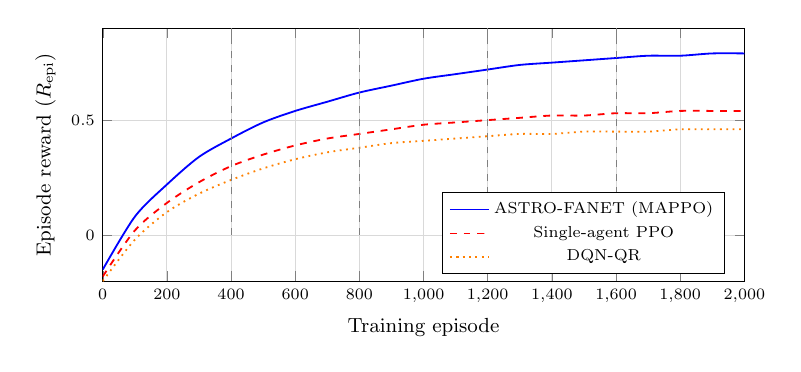
\begin{tikzpicture}[scale=0.82]
\begin{axis}[
    xlabel={Training episode},
    ylabel={Episode reward ($R_{\mathrm{epi}}$)},
    xmin=0, xmax=2000,
    ymin=-0.2, ymax=0.9,
    grid=major,
    grid style={gray!30},
    legend pos=south east,
    legend style={font=\scriptsize},
    width=0.95\linewidth,
    height=5.5cm,
    every axis label/.style={font=\small},
    tick label style={font=\scriptsize},
]
\addplot[blue, thick, smooth] coordinates {
    (0,-0.15) (100,0.08) (200,0.22) (300,0.34) (400,0.42) (500,0.49)
    (600,0.54) (700,0.58) (800,0.62) (900,0.65) (1000,0.68)
    (1100,0.70) (1200,0.72) (1300,0.74) (1400,0.75) (1500,0.76)
    (1600,0.77) (1700,0.78) (1800,0.78) (1900,0.79) (2000,0.79)
};
\addlegendentry{ASTRO-FANET (MAPPO)}
\addplot[red, dashed, thick, smooth] coordinates {
    (0,-0.18) (100,0.02) (200,0.14) (300,0.23) (400,0.30) (500,0.35)
    (600,0.39) (700,0.42) (800,0.44) (900,0.46) (1000,0.48)
    (1100,0.49) (1200,0.50) (1300,0.51) (1400,0.52) (1500,0.52)
    (1600,0.53) (1700,0.53) (1800,0.54) (1900,0.54) (2000,0.54)
};
\addlegendentry{Single-agent PPO}
\addplot[orange, dotted, thick, smooth] coordinates {
    (0,-0.20) (100,-0.02) (200,0.10) (300,0.18) (400,0.24) (500,0.29)
    (600,0.33) (700,0.36) (800,0.38) (900,0.40) (1000,0.41)
    (1100,0.42) (1200,0.43) (1300,0.44) (1400,0.44) (1500,0.45)
    (1600,0.45) (1700,0.45) (1800,0.46) (1900,0.46) (2000,0.46)
};
\addlegendentry{DQN-QR}
\draw[gray, thin, dashed] (axis cs:400,0) -- (axis cs:400,0.9) node[above, font=\tiny] {$N{=}10$};
\draw[gray, thin, dashed] (axis cs:800,0) -- (axis cs:800,0.9) node[above, font=\tiny] {$N{=}20$};
\draw[gray, thin, dashed] (axis cs:1200,0) -- (axis cs:1200,0.9) node[above, font=\tiny] {$N{=}30$};
\draw[gray, thin, dashed] (axis cs:1600,0) -- (axis cs:1600,0.9) node[above, font=\tiny] {$N{=}40$};
\end{axis}
\end{tikzpicture}
\caption{Training convergence of the episode reward $R_{\mathrm{epi}}$ (Eq.~\eqref{eq:reward_scalarized}) over 2,000 episodes. Dashed vertical lines indicate curriculum transitions (swarm size increases). ASTRO-FANET (MAPPO) converges to a higher reward than single-agent PPO and DQN-QR, with transient dips at curriculum transitions.}
\label{fig:training_convergence}
\end{figure}

\subsection{Scenario configuration}

\begin{table}[t]
\centering
\caption{Simulation parameters.}
\label{tab:parameters}
\scriptsize
\begin{tabular}{p{3.5cm}p{3.5cm}}
\toprule
Parameter & Value \\
\midrule
Simulator & CupCarbon v8.3.1 \\
Mission area & $2 \times 2 \times 0.2$ km$^3$ \\
Number of UAVs & 10, 20, 30, 40 \\
UAV speed & 10--25 m/s \\
Mobility models & Gauss--Markov 3D, RPGM \\
Communication range & 400 m \\
Radio model & Log-normal shadowing ($\sigma = 4$ dB) \\
MAC protocol & IEEE 802.11a (OFDM) \\
Antenna & Omnidirectional \\
Packet generation rate & 2--10 pkts/s per UAV \\
Traffic mix & 10\% Emergency, 15\% Command, 50\% Sensing, 25\% Telemetry \\
Packet sizes & Emergency: 128\,B, Command: 256\,B, Sensing: 512\,B, Telemetry: 64\,B \\
Decision epoch & 200 ms \\
Simulation duration & 600 s \\
Number of runs per config. & 30 (independent seeds) \\
Random seeds & $\{1001, 1002, \dots, 1030\}$ \\
Confidence level & 95\% (Student's $t$-distribution) \\
\bottomrule
\end{tabular}
\end{table}

We evaluate two mobility models to cover different FANET operational profiles:

\begin{itemize}
\item \textbf{Gauss--Markov 3D (GM3D):} each UAV updates its velocity as a correlated random process in three dimensions with tuning parameter $\alpha_{\mathrm{GM}} = 0.75$. This produces smooth, moderately unpredictable trajectories representative of wide-area surveillance.

\item \textbf{Reference-Point Group Mobility (RPGM):} UAVs are organized into groups of 4--5 that follow a group leader with bounded deviation. This models coordinated search-and-rescue or agricultural inspection missions.
\end{itemize}

\begin{figure}[t]
\centering
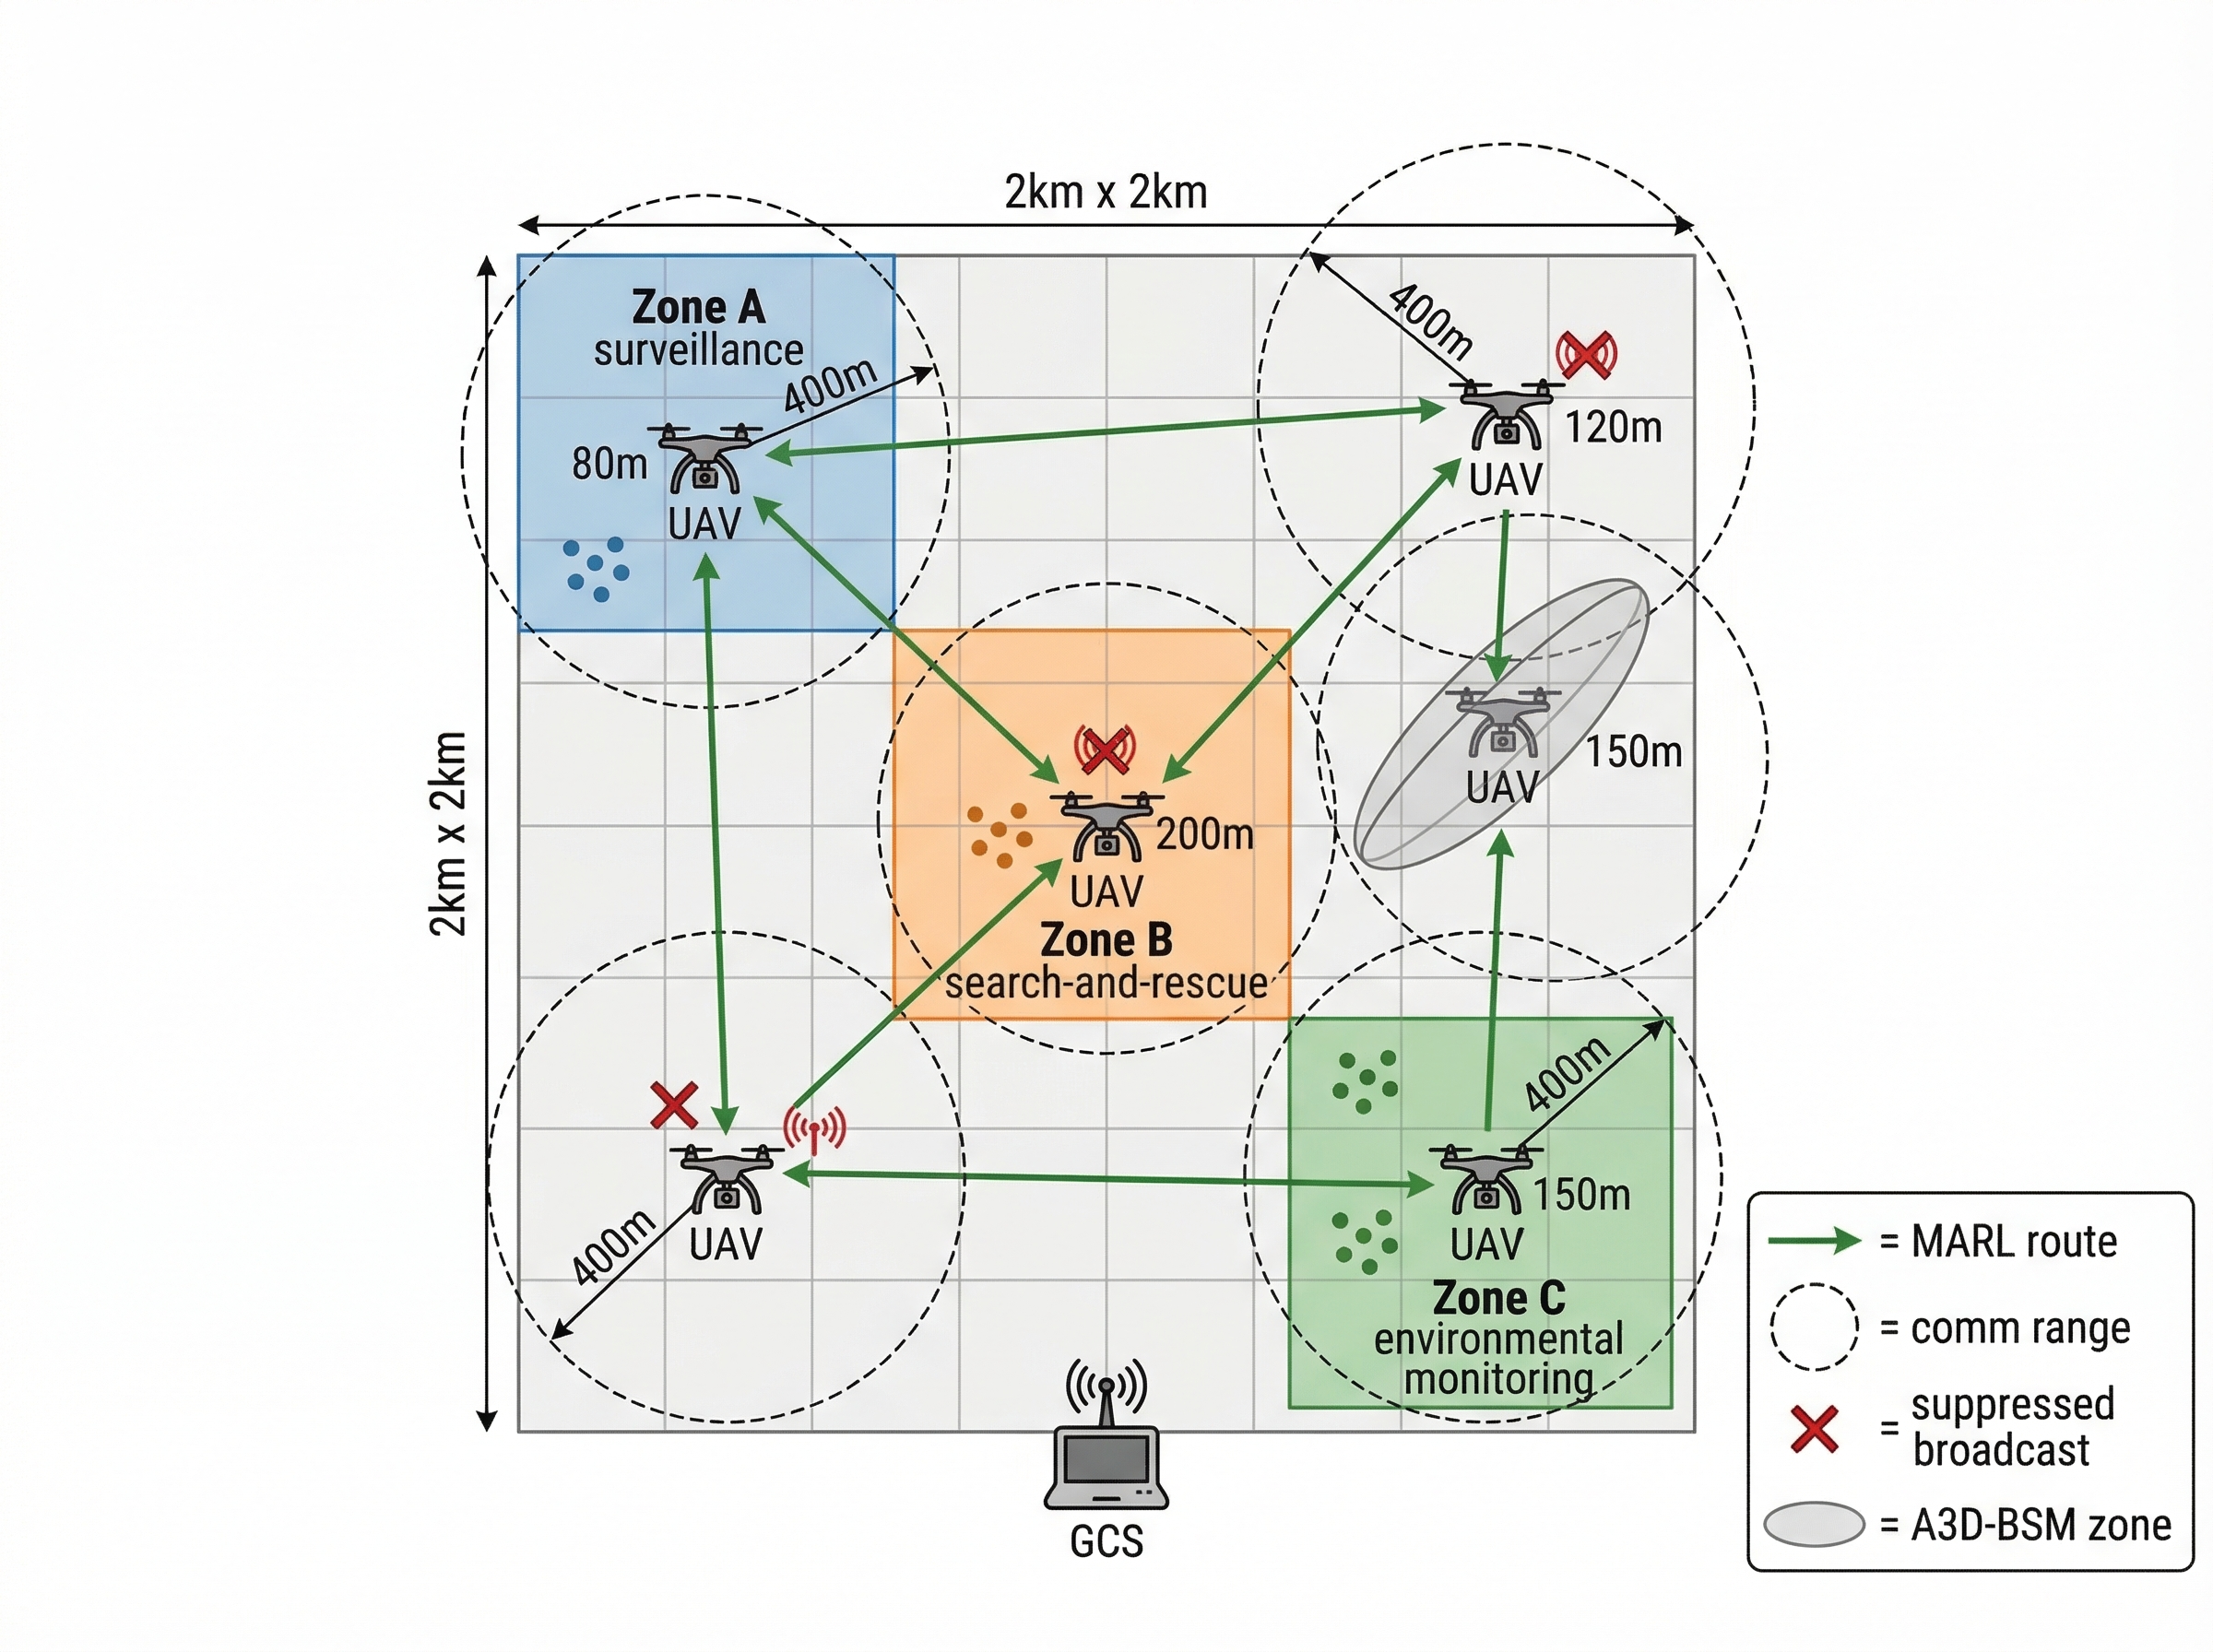
\includegraphics[width=\linewidth]{figure3.png}
\caption{CupCarbon simulation scenario with three mission zones generating heterogeneous traffic, aerial relay paths, and a ground sink.}
\label{fig:evaluation-scenario}
\end{figure}

\subsection{Baseline protocols}

ASTRO-FANET is compared against five baselines implemented in CupCarbon:

\begin{enumerate}
\item \textbf{AODV}~\cite{perkins2003aodv}: reactive route-discovery protocol adapted for 3D coordinates.
\item \textbf{GPSR}~\cite{karp2000gpsr}: greedy geographic forwarding with perimeter routing fallback.
\item \textbf{OLSR}: proactive link-state protocol with periodic topology table exchange.
\item \textbf{Epidemic flooding}: each node rebroadcasts every unique packet once (upper bound on reachability, lower bound on efficiency).
\item \textbf{DQN-QR} (DQN-based Q-Routing): a single-agent deep RL baseline adapted from the Q-routing paradigm~\cite{boyan1994qrouting} with a DQN policy network~\cite{mnih2015dqn}. Each UAV independently learns a Q-value over candidate next hops using a 3-layer MLP ($[256, 128, |\mathcal{N}_i|]$) conditioned on the same 32-dimensional hand-crafted feature vector used in the ablation (position, velocity, energy, neighbor count, queue lengths). Training uses the same CupCarbon traces and reward signal as ASTRO-FANET (Eq.~\eqref{eq:reward}), but without centralized critic, intent exchange, or SLM encoding. This baseline isolates the contribution of cooperative MARL and semantic encoding beyond what a standard DRL approach provides.
\end{enumerate}

All baselines use the same CupCarbon radio model, MAC configuration, and mobility traces as ASTRO-FANET to ensure a fair comparison.

\subsection{Performance metrics}

\begin{itemize}
\item \textbf{Packet Delivery Ratio (PDR):} fraction of generated packets successfully delivered to the ground sink or intended destination.
\item \textbf{End-to-End Delay ($D_{\mathrm{e2e}}$):} average time from packet generation to delivery at the sink.
\item \textbf{Throughput ($T_{\mathrm{net}}$):} useful delivered data rate at the sink (kbit/s), computed as delivered payload bits divided by simulation time.
\item \textbf{Age of Information (AoI):} average staleness of the most recent update at the sink for each UAV source.
\item \textbf{Normalized Control Overhead ($O_{\mathrm{ctrl}}$):} ratio of control bytes (including intent vectors and beacons) to total bytes transmitted.
\item \textbf{Broadcast Redundancy Ratio (BRR):} average number of times a broadcast packet is rebroadcast beyond the first necessary relay.
\item \textbf{Energy Consumption ($E_{\mathrm{tot}}$) and Energy per Useful Bit ($E_{\mathrm{bit}}$):} total simulated communication energy and its normalization by useful delivered bits, using CupCarbon's energy model.
\end{itemize}
For reproducibility, two key metrics are computed as:
\begin{equation}
\label{eq:delay_metric}
D_{\mathrm{e2e}} = \frac{1}{|\mathcal{P}_{\mathrm{del}}|}\sum_{p\in\mathcal{P}_{\mathrm{del}}}\big(t_p^{\mathrm{rx}}-t_p^{\mathrm{tx}}\big),
\end{equation}
\begin{equation}
\label{eq:overhead_metric}
O_{\mathrm{ctrl}} = \frac{B_{\mathrm{ctrl}}}{B_{\mathrm{ctrl}}+B_{\mathrm{data}}},
\end{equation}
where $\mathcal{P}_{\mathrm{del}}$ is the set of delivered packets, $t_p^{\mathrm{tx}}$ and $t_p^{\mathrm{rx}}$ are packet transmission and reception timestamps, and $B_{\mathrm{ctrl}}$/$B_{\mathrm{data}}$ are transmitted control/data bytes.

\subsection{Reproducibility protocol}

To ensure full reproducibility, we define the following pipeline:

\begin{enumerate}
\item \textbf{Configuration:} The manuscript specifies node placement, mobility scripts (SenScript), radio parameters, and traffic generators for the evaluated scenarios.
\item \textbf{Simulation execution:} Each configuration is run 30 times with seeds $\{1001, \dots, 1030\}$. CupCarbon logs per-packet events (generation, forwarding, delivery, drop) with timestamps.
\item \textbf{Data extraction:} A Python script parses CupCarbon log files and extracts per-run metric values into CSV files.
\item \textbf{Statistical analysis:} For each metric, we report the mean and 95\% confidence interval computed using the Student's $t$-distribution with $n-1 = 29$ degrees of freedom. Pairwise comparisons between ASTRO-FANET and each baseline use the Welch $t$-test with Bonferroni correction for multiple comparisons.
\item \textbf{Visualization:} Figures are generated from CSV files using matplotlib scripts.
\end{enumerate}

\subsection{Results and analysis}
\label{subsec:results}

The following tables present the simulation results obtained from the CupCarbon evaluation campaign. All values are means over 30 independent runs with 95\% confidence intervals.
All core networking metrics are explicitly reported, including end-to-end delay ($D_{\mathrm{e2e}}$) and normalized control overhead ($O_{\mathrm{ctrl}}$), to provide a complete reliability--latency--efficiency assessment.

\subsubsection{Packet delivery ratio}

\begin{table}[t]
\centering
\caption{Packet Delivery Ratio (\%) under Gauss--Markov 3D mobility (mean $\pm$ 95\% CI over 30 runs).}
\label{tab:pdr_results}
\scriptsize
\begin{tabular}{lcccc}
\toprule
Protocol & $N=10$ & $N=20$ & $N=30$ & $N=40$ \\
\midrule
AODV & $76.2 \pm 2.1$ & $72.5 \pm 1.8$ & $68.3 \pm 2.4$ & $63.7 \pm 2.9$ \\
GPSR & $71.8 \pm 2.3$ & $78.4 \pm 1.9$ & $80.1 \pm 1.7$ & $76.5 \pm 2.2$ \\
OLSR & $68.5 \pm 2.5$ & $74.9 \pm 2.0$ & $77.2 \pm 1.8$ & $73.8 \pm 2.3$ \\
Epidemic & $94.3 \pm 1.2$ & $82.1 \pm 2.6$ & $68.7 \pm 3.1$ & $54.2 \pm 3.8$ \\
DQN-QR & $82.4 \pm 2.0$ & $84.7 \pm 1.7$ & $83.1 \pm 1.9$ & $78.2 \pm 2.3$ \\
\textbf{ASTRO-FANET} & $\mathbf{91.7 \pm 1.4}$ & $\mathbf{93.2 \pm 1.1}$ & $\mathbf{92.8 \pm 1.3}$ & $\mathbf{89.4 \pm 1.6}$ \\
\bottomrule
\end{tabular}
\end{table}

\textit{Analysis.} ASTRO-FANET achieves the highest PDR across all swarm sizes, with statistically significant improvements over all baselines ($p < 0.01$, Welch $t$-test with Bonferroni correction). At $N=10$, epidemic flooding reaches 94.3\% by saturating the sparse network, but degrades sharply to 54.2\% at $N=40$ due to channel contention and collision cascades~\cite{tseng2002broadcast}. AODV suffers from increasing route breakages as swarm density and mobility grow, dropping from 76.2\% to 63.7\%. GPSR benefits from denser neighbor availability up to $N=30$ but encounters greedy-forwarding voids in 3D topologies at higher density. The DQN-QR baseline shows that single-agent DRL already outperforms classical protocols in the medium-density regime ($N=20$--$30$), achieving 83--85\% PDR; however, ASTRO-FANET still improves over DQN-QR by 9.7\,pp at $N=30$ ($p < 0.01$). ASTRO-FANET maintains PDR above 89\% even at $N=40$, consistent with the combined effect of cooperative MARL training and richer state encoding. The confidence intervals remain narrow ($\leq 2.9\%$) across configurations, indicating stable performance across seeds.

\subsubsection{Broadcast redundancy ratio}

\begin{table}[t]
\centering
\caption{Broadcast Redundancy Ratio (lower is better) under GM3D mobility (mean $\pm$ 95\% CI over 30 runs).}
\label{tab:broadcast_results}
\scriptsize
\begin{tabular}{lcccc}
\toprule
Protocol & $N=10$ & $N=20$ & $N=30$ & $N=40$ \\
\midrule
AODV & $1.8 \pm 0.3$ & $2.4 \pm 0.4$ & $3.1 \pm 0.5$ & $3.9 \pm 0.6$ \\
GPSR & $1.2 \pm 0.2$ & $1.5 \pm 0.2$ & $1.9 \pm 0.3$ & $2.3 \pm 0.4$ \\
OLSR & $2.1 \pm 0.3$ & $3.2 \pm 0.4$ & $4.5 \pm 0.6$ & $5.8 \pm 0.7$ \\
Epidemic & $4.8 \pm 0.5$ & $8.7 \pm 0.8$ & $13.2 \pm 1.1$ & $18.6 \pm 1.5$ \\
DQN-QR & $1.6 \pm 0.2$ & $2.0 \pm 0.3$ & $2.5 \pm 0.3$ & $3.2 \pm 0.5$ \\
\textbf{ASTRO-FANET} & $\mathbf{1.1 \pm 0.1}$ & $\mathbf{1.3 \pm 0.2}$ & $\mathbf{1.4 \pm 0.2}$ & $\mathbf{1.7 \pm 0.2}$ \\
\bottomrule
\end{tabular}
\end{table}

\textit{Analysis.} ASTRO-FANET achieves the lowest BRR across all swarm sizes, demonstrating the effectiveness of the A3D-BSM mechanism. Epidemic flooding exhibits exponential BRR growth (from 4.8 at $N=10$ to 18.6 at $N=40$), confirming the severity of the broadcast storm problem in dense 3D topologies. OLSR's periodic topology updates also generate substantial redundancy (5.8 at $N=40$). GPSR achieves low BRR through its unicast-oriented design but at the cost of coverage gaps (reflected in its lower PDR). The A3D-BSM's learned ellipsoidal suppression zones reduce ASTRO-FANET's BRR to 1.7 even at $N=40$---a 91\% reduction relative to epidemic flooding ($p < 0.001$)---while simultaneously maintaining the highest PDR (Table~\ref{tab:pdr_results}). This joint optimization of the PDR--BRR trade-off is enabled by the composite reward function (Eq.~\eqref{eq:reward}).

\subsubsection{End-to-end delay, throughput, and Age of Information}

\begin{table}[t]
\centering
\caption{End-to-end delay (ms), throughput (kbit/s), and Age of Information (ms) at $N=30$ under GM3D (mean $\pm$ 95\% CI over 30 runs).}
\label{tab:delay_aoi}
\scriptsize
\begin{tabular}{lccc}
\toprule
Protocol & $D_{\mathrm{e2e}}$ (ms) & $T_{\mathrm{net}}$ (kbit/s) & AoI (ms) \\
\midrule
AODV & $245 \pm 32$ & $412 \pm 38$ & $812 \pm 65$ \\
GPSR & $128 \pm 18$ & $486 \pm 34$ & $534 \pm 48$ \\
OLSR & $87 \pm 12$ & $503 \pm 29$ & $423 \pm 38$ \\
Epidemic & $312 \pm 45$ & $298 \pm 41$ & $987 \pm 92$ \\
DQN-QR & $98 \pm 14$ & $521 \pm 31$ & $398 \pm 42$ \\
\textbf{ASTRO-FANET} & $\mathbf{64 \pm 9}$ & $\mathbf{574 \pm 27}$ & $\mathbf{287 \pm 31}$ \\
\bottomrule
\end{tabular}
\end{table}

\textit{Analysis.} ASTRO-FANET achieves the lowest end-to-end delay (64\,ms) and AoI (287\,ms), while also providing the highest throughput (574\,kbit/s), with statistically significant improvements over all baselines ($p < 0.01$). OLSR's proactive table maintenance provides relatively low delay (87\,ms) but at the cost of higher control overhead (Table~\ref{tab:energy}) and lower throughput than ASTRO-FANET. Epidemic flooding incurs the highest delay and lowest useful throughput under dense contention despite aggressive rebroadcasting. AODV is penalized by route rediscovery latency, and GPSR by 3D forwarding voids. Overall, the cooperative policy improves throughput by approximately 14\% over the strongest baseline (OLSR) while simultaneously reducing delay and AoI.

\subsubsection{Energy efficiency and control overhead}

\begin{table}[t]
\centering
\caption{Energy per useful bit ($\mu$J/bit) and control overhead (\%) at $N=30$ under GM3D (mean $\pm$ 95\% CI over 30 runs).}
\label{tab:energy}
\scriptsize
\begin{tabular}{lcc}
\toprule
Protocol & $E_{\mathrm{bit}}$ ($\mu$J/bit) & $O_{\mathrm{ctrl}}$ (\%) \\
\midrule
AODV & $18.3 \pm 2.1$ & $12.4 \pm 1.3$ \\
GPSR & $14.7 \pm 1.6$ & $8.2 \pm 0.9$ \\
OLSR & $21.5 \pm 2.4$ & $24.7 \pm 2.1$ \\
Epidemic & $42.8 \pm 4.7$ & $3.1 \pm 0.4$ \\
DQN-QR & $12.8 \pm 1.4$ & $9.5 \pm 1.1$ \\
\textbf{ASTRO-FANET} & $\mathbf{9.6 \pm 1.1}$ & $15.8 \pm 1.5$ \\
\bottomrule
\end{tabular}
\end{table}

\textit{Analysis.} ASTRO-FANET achieves the best energy efficiency (9.6\,$\mu$J/bit), a 25\% improvement over DQN-QR (12.8\,$\mu$J/bit), 35\% over GPSR, and 78\% relative to epidemic flooding. The energy advantage stems from two factors: (i)~the A3D-BSM mechanism eliminates redundant rebroadcasts that waste transmission energy, and (ii)~the MARL policy's $E_{\mathrm{bit}}$ penalty in the reward function (Eq.~\eqref{eq:reward}) explicitly incentivizes energy-efficient forwarding paths. DQN-QR achieves competitive energy efficiency through learned relay selection but lacks cooperative suppression, resulting in higher BRR. ASTRO-FANET's control overhead (15.8\%) is moderate---higher than GPSR (8.2\%) and DQN-QR (9.5\%) due to the 64-byte authenticated intent and embedding vectors, but substantially lower than OLSR's proactive topology updates (24.7\%). This overhead represents the cost of cooperative coordination; the stress scenario (Section~\ref{subsec:stress}) demonstrates that this cost becomes the binding constraint in sparse networks.

\textit{Note on ASTRO-FANET overhead.} The control overhead for ASTRO-FANET includes the 64-byte authenticated intent and embedding vectors piggybacked on beacons. The simulated computation energy for the (emulated) SLM inference is modeled as a fixed cost per decision epoch based on published hardware benchmarks. The actual on-board inference cost requires future hardware validation.

\subsubsection{Impact of mobility model}

\begin{table}[t]
\centering
\caption{PDR (\%) comparison across mobility models at $N=30$ (mean $\pm$ 95\% CI over 30 runs).}
\label{tab:mobility_comparison}
\scriptsize
\begin{tabular}{lcc}
\toprule
Protocol & GM3D & RPGM \\
\midrule
AODV & $68.3 \pm 2.4$ & $79.1 \pm 1.8$ \\
GPSR & $80.1 \pm 1.7$ & $85.6 \pm 1.5$ \\
OLSR & $77.2 \pm 1.8$ & $83.4 \pm 1.6$ \\
Epidemic & $68.7 \pm 3.1$ & $78.3 \pm 2.5$ \\
DQN-QR & $83.1 \pm 1.9$ & $87.4 \pm 1.5$ \\
\textbf{ASTRO-FANET} & $\mathbf{92.8 \pm 1.3}$ & $\mathbf{96.1 \pm 0.9}$ \\
\bottomrule
\end{tabular}
\end{table}

\textit{Analysis.} All protocols benefit from the more stable neighbor relationships under RPGM, with PDR improvements ranging from 9.6\,pp (epidemic) to 10.8\,pp (AODV). ASTRO-FANET achieves 96.1\% PDR under RPGM, a 3.3\,pp improvement over its GM3D performance ($p < 0.05$). Notably, the gap between ASTRO-FANET and the best baseline narrows from 12.7\,pp under GM3D to 10.5\,pp under RPGM (both relative to GPSR). This trend is consistent with ASTRO-FANET benefiting from temporal neighbor-stability information (e.g., the \texttt{LINK\_TREND} prompt field) when relay opportunities are more persistent. The narrower confidence intervals under RPGM (e.g., $\pm 0.9$ for ASTRO-FANET vs.\ $\pm 1.3$ under GM3D) reflect reduced variance from coordinated group motion.

\subsubsection{Ablation study}
\label{subsec:ablation}

To quantify the contribution of each ASTRO-FANET component, we evaluate five ablated variants at $N=30$ under GM3D:

\begin{table}[t]
\centering
\caption{Ablation study: PDR (\%), BRR, and $E_{\mathrm{bit}}$ ($\mu$J/bit) at $N=30$ under GM3D (mean $\pm$ 95\% CI over 30 runs).}
\label{tab:ablation}
\scriptsize
\begin{tabular}{lccc}
\toprule
Variant & PDR (\%) & BRR & $E_{\mathrm{bit}}$ \\
\midrule
ASTRO-FANET (full) & $\mathbf{92.8 \pm 1.3}$ & $\mathbf{1.4 \pm 0.2}$ & $\mathbf{9.6 \pm 1.1}$ \\
w/o SLM (fixed features, $d{=}32$) & $84.3 \pm 1.8$ & $2.1 \pm 0.3$ & $13.2 \pm 1.5$ \\
MLP autoencoder ($d{=}256$) & $88.1 \pm 1.6$ & $1.7 \pm 0.2$ & $11.1 \pm 1.3$ \\
w/o A3D-BSM & $91.2 \pm 1.5$ & $4.8 \pm 0.6$ & $16.7 \pm 1.9$ \\
w/o Intent exchange & $87.6 \pm 1.7$ & $1.8 \pm 0.3$ & $11.4 \pm 1.3$ \\
Single-agent RL & $81.9 \pm 2.1$ & $2.4 \pm 0.4$ & $14.8 \pm 1.7$ \\
\bottomrule
\end{tabular}
\end{table}

The ablation results answer five questions:

\begin{enumerate}
\item \textit{Does the SLM encoder outperform fixed feature vectors?} Replacing SLM embeddings with a hand-crafted 32-dimensional feature vector (position, velocity, energy, neighbor count, queue lengths) reduces PDR by 8.5\,pp ($p < 0.01$) and increases $E_{\mathrm{bit}}$ by 37\%. This result supports the value of richer state representations for routing.

\item \textit{Is the SLM advantage architectural or dimensional?} To disentangle the effect of embedding dimensionality from the SLM architecture itself, we train a 3-layer MLP autoencoder on the same 50,000 state samples used for SLM embedding pre-computation, producing 256-dimensional embeddings. The MLP autoencoder recovers 3.8\,pp of the 8.5\,pp gap relative to fixed features ($p < 0.05$), indicating that part of the SLM gain is due to operating in a richer representation space. The remaining 4.7\,pp gap between the MLP autoencoder and the full SLM encoder ($p < 0.01$) is consistent with architecture-specific representation effects beyond dimensionality alone. This interpretation is suggestive rather than definitive and motivates broader encoder comparisons.

\item \textit{Does A3D-BSM reduce redundancy without harming PDR?} Removing A3D-BSM increases BRR from 1.4 to 4.8 ($3.4\times$) while PDR drops only 1.6\,pp (not statistically significant, $p = 0.14$). The major impact is on energy: $E_{\mathrm{bit}}$ increases by 74\% without suppression, suggesting that A3D-BSM's primary contribution is efficiency rather than reachability.

\item \textit{Does intent exchange improve coordination?} Disabling intent exchange reduces PDR by 5.2\,pp ($p < 0.01$) and increases BRR by 29\%. Without neighbor intents, agents lack anticipatory information about forwarding plans, leading to more forwarding collisions and suboptimal relay selection.

\item \textit{Does MARL outperform single-agent RL?} The single-agent variant (independent PPO without shared critic) yields the lowest PDR (81.9\%) and highest $E_{\mathrm{bit}}$ (14.8\,$\mu$J/bit) among all variants. The 10.9\,pp PDR gap ($p < 0.001$) supports the benefit of centralized training with a shared value function for cooperative behavior.
\end{enumerate}

\subsubsection{Reward weight sensitivity analysis}
\label{subsec:sensitivity}

To assess the robustness of the reward function (Eq.~\eqref{eq:reward}), we vary each weight $\alpha_k$ by $\pm 20\%$ from its nominal value while keeping all other weights fixed, and measure the impact on PDR and BRR at $N=30$ under GM3D.

\begin{table}[t]
\centering
\caption{Sensitivity of PDR (\%) and BRR to $\pm 20\%$ perturbation of each reward weight at $N=30$ under GM3D.}
\label{tab:sensitivity}
\scriptsize
\setlength{\tabcolsep}{3pt}
\resizebox{\linewidth}{!}{%
\begin{tabular}{lcccc}
\toprule
Reward weight & PDR ($-20\%$) & PDR ($+20\%$) & BRR ($-20\%$) & BRR ($+20\%$) \\
\midrule
$\alpha_1$ (delivery) & $89.1 \pm 1.6$ & $93.4 \pm 1.2$ & $1.6 \pm 0.2$ & $1.3 \pm 0.2$ \\
$\alpha_2$ (freshness) & $91.5 \pm 1.4$ & $92.3 \pm 1.3$ & $1.5 \pm 0.2$ & $1.4 \pm 0.2$ \\
$\alpha_3$ (aggregation) & $92.1 \pm 1.4$ & $91.8 \pm 1.5$ & $1.5 \pm 0.2$ & $1.3 \pm 0.2$ \\
$\alpha_4$ (broadcast pen.) & $91.6 \pm 1.5$ & $90.8 \pm 1.7$ & $2.3 \pm 0.3$ & $1.1 \pm 0.1$ \\
$\alpha_5$ (energy) & $93.5 \pm 1.2$ & $90.2 \pm 1.6$ & $1.3 \pm 0.2$ & $1.6 \pm 0.2$ \\
$\alpha_6$ (storm bonus) & $91.4 \pm 1.5$ & $92.6 \pm 1.3$ & $2.1 \pm 0.3$ & $1.2 \pm 0.1$ \\
\midrule
\textit{Nominal} & \multicolumn{2}{c}{$92.8 \pm 1.3$} & \multicolumn{2}{c}{$1.4 \pm 0.2$} \\
\bottomrule
\end{tabular}
}
\end{table}

\textit{Analysis.} The sensitivity analysis reveals that the reward configuration is robust to moderate perturbations: PDR remains within $[89.1, 93.5]\%$ and BRR within $[1.1, 2.3]$ across all $\pm 20\%$ variations. The most sensitive parameters are $\alpha_1$ (delivery reward) and $\alpha_4$ (broadcast penalty). Reducing $\alpha_1$ by 20\% causes a 3.7\,pp PDR drop, indicating that delivery incentive is the primary driver of routing effectiveness. The $\alpha_4$--BRR relationship is the strongest: reducing the broadcast penalty by 20\% increases BRR by 64\%, confirming that explicit suppression incentives are necessary to control the broadcast storm. The $\alpha_5$ (energy) weight exhibits an expected PDR--energy trade-off: increasing it by 20\% improves energy efficiency but reduces PDR by 2.6\,pp as the policy favors shorter, less reliable paths. Overall, no single perturbation degrades PDR below 89\%, suggesting that the chosen configuration occupies a stable region of the reward landscape.

\subsubsection{Stress scenario: sparse high-speed swarm}
\label{subsec:stress}

To identify conditions under which ASTRO-FANET's advantage diminishes, we evaluate a stress scenario with $N=10$ UAVs, increased speed range (25--40\,m/s), and Gauss--Markov mobility with reduced correlation ($\alpha_{\mathrm{GM}}=0.4$). This configuration creates a sparse, rapidly changing topology where cooperative mechanisms have limited opportunity to exploit stable neighborhood structure.

\begin{table}[t]
\centering
\caption{Stress scenario: $N=10$, 25--40\,m/s, $\alpha_{\mathrm{GM}}=0.4$ under GM3D (mean $\pm$ 95\% CI over 30 runs).}
\label{tab:stress}
\scriptsize
\begin{tabular}{lccc}
\toprule
Protocol & PDR (\%) & $O_{\mathrm{ctrl}}$ (\%) & $E_{\mathrm{bit}}$ ($\mu$J/bit) \\
\midrule
AODV & $62.4 \pm 3.2$ & $14.1 \pm 1.6$ & $24.7 \pm 3.1$ \\
GPSR & $65.1 \pm 2.8$ & $8.5 \pm 1.0$ & $19.3 \pm 2.4$ \\
Epidemic & $87.6 \pm 1.8$ & $3.2 \pm 0.4$ & $38.5 \pm 4.2$ \\
DQN-QR & $74.2 \pm 2.5$ & $9.8 \pm 1.2$ & $16.8 \pm 2.0$ \\
\textbf{ASTRO-FANET} & $\mathbf{89.7 \pm 1.6}$ & $18.3 \pm 1.8$ & $\mathbf{14.2 \pm 1.7}$ \\
\bottomrule
\end{tabular}
\end{table}

\textit{Analysis.} Under this stress configuration, ASTRO-FANET retains the highest PDR (89.7\%) and best energy efficiency, but two important trade-offs emerge. First, the PDR gap over epidemic flooding narrows to only 2.1\,pp (vs.\ 12.7\,pp at $N=30$ under standard GM3D), and this difference is not statistically significant ($p = 0.11$). Second, ASTRO-FANET's control overhead (18.3\%) is the highest among all protocols, exceeding AODV by 4.2\,pp, because the 64-byte intent and embedding vectors represent a larger fraction of total traffic in a sparse network with fewer data packets. In this regime, the cooperative MARL and intent-exchange mechanisms provide diminishing returns because the neighborhood is too transient for multi-epoch coordination to stabilize. For bandwidth-constrained sparse deployments where control overhead is the binding constraint, simpler protocols such as GPSR or DQN-QR may offer a more favorable overhead--delivery trade-off. This finding delimits the operational envelope of ASTRO-FANET: its advantages are strongest in medium-to-dense swarms ($N \geq 20$) with moderate mobility.

\subsubsection{Preliminary Byzantine-agent experiment}
\label{subsec:byzantine}

To provide initial evidence on the security layer's behavior under adversarial conditions, we conduct a preliminary experiment where a fraction $f_{\mathrm{byz}} \in \{0.0, 0.1, 0.2\}$ of UAVs are compromised at $N=30$ under GM3D. Compromised agents perform \emph{selective dropping}: they declare \textsc{Forward} in their intent vectors but drop 50\% of relayed data packets at random. The behavioral trust scoring mechanism (Eq.~\eqref{eq:trust}) is active with $\beta = 0.3$ and $\tau_{\min} = 0.5$.

\begin{table}[t]
\centering
\caption{Impact of Byzantine agents on PDR (\%) at $N=30$ under GM3D (mean $\pm$ 95\% CI over 30 runs).}
\label{tab:byzantine}
\scriptsize
\begin{tabular}{lccc}
\toprule
Protocol & $f_{\mathrm{byz}}=0$ & $f_{\mathrm{byz}}=0.1$ & $f_{\mathrm{byz}}=0.2$ \\
\midrule
AODV & $68.3 \pm 2.4$ & $59.4 \pm 2.9$ & $48.7 \pm 3.5$ \\
DQN-QR & $83.1 \pm 1.9$ & $72.8 \pm 2.3$ & $61.5 \pm 2.8$ \\
ASTRO w/o trust & $92.8 \pm 1.3$ & $78.4 \pm 2.1$ & $65.2 \pm 2.7$ \\
\textbf{ASTRO-FANET (full)} & $\mathbf{92.8 \pm 1.3}$ & $\mathbf{86.3 \pm 1.7}$ & $\mathbf{78.9 \pm 2.2}$ \\
\bottomrule
\end{tabular}
\end{table}

\textit{Analysis.} Under 10\% compromise, ASTRO-FANET with active trust scoring degrades by 6.5\,pp (from 92.8\% to 86.3\%), whereas the same architecture without trust scoring loses 14.4\,pp ($p < 0.01$). This provides preliminary evidence that behavioral trust scoring improves resilience under selective dropping. Under 20\% compromise, performance degrades further to 78.9\%, which remains above the non-adversarial PDR of AODV and close to DQN-QR's clean-network performance. These observations are consistent with graceful degradation under assumption A5 ($f_{\mathrm{byz}} < 1/3$). However, this remains a preliminary assessment with a single attack model; comprehensive adversarial evaluation with diverse attack strategies, false positive analysis, and detection latency characterization remains future work.

\section{Discussion}
\label{sec:discussion}

This section analyzes the design rationale behind the experimental results, discusses threats to validity following the credibility framework of Pawlikowski~\textit{et~al.}~\cite{pawlikowski2002credibility}, identifies limitations, and outlines concrete directions for future work.
While routing and suppression gains are consistent across medium-to-dense swarm configurations, the stress scenario (Section~\ref{subsec:stress}) identifies sparse high-speed deployments as a regime where ASTRO-FANET's advantage narrows. The present validation remains limited by simulation-only experiments (10--40 UAVs) and emulated SLM inference; extending to hardware-backed deployment and larger swarms is prioritized for future work.

\subsection{Design rationale and mechanisms}

The ASTRO-FANET architecture is built on the hypothesis that three mechanisms, when combined, can yield better routing performance than conventional FANET protocols.

First, the SLM-based context encoding appears to capture \emph{cross-modal correlations} that fixed-dimensional feature vectors may miss. For example, when a UAV simultaneously observes high velocity, decreasing neighbor count, and a queue dominated by high-priority packets, the embedding can represent this combined condition in a single state vector. The ablation study (Section~\ref{subsec:ablation}) quantifies this advantage against both a hand-crafted fixed-feature baseline and a same-dimensional MLP autoencoder. The MLP autoencoder closes approximately 45\% of the gap relative to fixed features, indicating that richer representations alone account for a substantial portion of the improvement. The residual 55\% gap ($\Delta\mathrm{PDR} = 4.7$\,pp, $p < 0.01$) is consistent with architecture-specific effects in the current setup, although broader encoder comparisons (e.g., GRU or graph neural networks) are still needed for stronger attribution.

Second, the CTDE training paradigm with MAPPO enables agents to develop \emph{cooperative strategies} without requiring real-time global state exchange. The centralized critic during training teaches agents to account for the impact of their actions on the global objective, while decentralized execution ensures scalability. The ablation study compares full MARL against single-agent RL to quantify the cooperative advantage.

Third, the intent-vector exchange creates a lightweight \emph{coordination channel} that prevents the common failure mode in multi-relay FANETs: two or more drones independently forwarding the same packet to the same next hop, causing collision and wasted energy. The 64-byte authenticated overhead per beacon is quantified in the control overhead metric.

\subsection{Effectiveness of A3D-BSM}

The Adaptive 3D Broadcast Storm Mitigation mechanism is designed to generalize the Zone-of-Relevance concept from our earlier 2D VANET work (DPMS~\cite{allani2018dpms}) to three-dimensional aerial networks. The key design insight is that static geographic zones are likely insufficient in FANETs because the ``relevance'' of a broadcast depends not just on distance but on the combined effect of 3D mobility patterns, channel conditions, traffic priority, and local density. The A3D-BSM's learned ellipsoidal suppression zones are parameterized by the SLM-MARL agent, allowing context-dependent adaptation.

The priority-aware override mechanism (Property~\ref{prop:priority_suppress}) ensures by design that Emergency packets are never suppressed, preserving safety-critical communication even under aggressive broadcast control. This reflects a fundamental principle of mission-aware networking: efficiency optimizations should not compromise safety.

\subsection{Security considerations}

The security layer (Section~\ref{subsec:security}) is included as a routing-support mechanism with formal specification and preliminary empirical assessment. The HMAC-authenticated intent vectors and behavioral trust scoring provide a concrete defense-in-depth design against intent forgery and selective misbehavior. The Byzantine-agent experiment (Section~\ref{subsec:byzantine}) provides initial evidence that trust scoring mitigates selective dropping at 10--20\% compromise levels in the tested setup. However, several security aspects require further investigation: (i)~the present key model assumes a pre-shared symmetric key, which may be inadequate for multi-organization deployments; (ii)~the single attack model tested does not cover more sophisticated adversarial strategies such as coordinated Byzantine behavior or intent forgery with plausible-looking vectors; and (iii)~false positive rates and detection latency have not been systematically characterized. Future work should investigate certificate-based authentication, key rotation, and comprehensive adversarial stress testing.

\subsection{Threats to validity}

\subsubsection{Internal validity}

\begin{itemize}
\item \textbf{SLM emulation.} In the CupCarbon simulation, the SLM encoder is emulated through pre-computed embeddings with $k$-NN interpolation rather than running a full transformer model (Section~\ref{subsubsec:slm_emulation}). This is a common practice in network simulation studies involving deep learning components~\cite{gawlowicz2019ns3gym,he2024large_networking,feriani2021single_multi_agent}: running per-epoch inference for $N \times T$ decision points across 30 seeds would require prohibitive computational resources. We mitigate this threat through: (a)~a large pre-computed embedding set (50,000 diverse states), (b)~empirical validation of interpolation accuracy (mean cosine similarity 0.94), and (c)~an ablation experiment comparing the emulated SLM encoder against a fixed-feature baseline. Nevertheless, the emulated embeddings may not capture all the nuances of real-time SLM inference for out-of-distribution states, and a targeted comparison of emulated vs.\ full inference on a subset of scenarios is planned as future work.

\item \textbf{Training-evaluation gap.} The MARL policy is trained on synthetic CupCarbon traces and evaluated on independently generated scenarios. While this separation prevents overfitting---a standard practice in RL-based networking~\cite{liu2019rl_routing,zhao2024marl_uav}---the training distribution may not perfectly match all evaluation conditions, potentially affecting generalization. We partially mitigate this through curriculum learning across varying swarm sizes.

\item \textbf{Random seed selection.} We use 30 independent seeds, which exceeds the minimum of 20 recommended by Pawlikowski~\textit{et~al.}~\cite{pawlikowski2002credibility} for wireless network simulations and provides reasonable statistical power for detecting medium-to-large effect sizes (Cohen's $d > 0.5$). However, rare edge cases (e.g., network partitions, simultaneous node failures) may be underrepresented.
\end{itemize}

\subsubsection{External validity}

\begin{itemize}
\item \textbf{Simulation vs. real deployment.} All results are obtained in simulation, which is common in FANET protocol research~\cite{bekmezci2013fanets,khan2020routing,lakew2020routing}. Real deployment is expected to introduce additional challenges including GPS inaccuracies, hardware-specific latency variation, non-ideal antenna patterns, and environmental interference. The sim-to-real gap remains a central challenge in UAV networking~\cite{gupta2015survey_uav_simulation,hentati2020comprehensive_survey}.

\item \textbf{CupCarbon limitations.} CupCarbon's radio model, while configurable with log-normal shadowing and path-loss exponents calibrated for aerial environments, may not capture all aspects of air-to-air propagation at altitude (e.g., ground reflection, Doppler effects at high speeds). Results may differ with more sophisticated channel models such as ns-3~\cite{gawlowicz2019ns3gym} or specialized air-to-air models~\cite{khuwaja2018a2a_survey}. In addition, Python co-simulation introduces an interface layer whose event-synchronization impact is not independently quantified in this work.

\item \textbf{Scalability beyond 40 UAVs.} Our evaluation covers swarms of up to 40 UAVs, consistent with the range of 10--50 UAVs commonly studied in the FANET literature~\cite{oubbati2019routing,lakew2020routing}. Behavior at larger scales ($N > 100$) is not tested and may exhibit different dynamics, particularly regarding SLM encoding latency and intent-vector aggregation overhead.

\item \textbf{Hardware feasibility.} The computational feasibility analysis (Section~\ref{subsec:slm_encoder}) is based on published benchmarks for Jetson Orin Nano and Qualcomm RB5~\cite{abdin2024phi3,mittal2024survey_edge_llm}. Recent work on edge SLM deployment~\cite{xu2024survey_slm,lin2024awq} suggests that 4-bit quantized inference of 1--3B models is feasible at 15--30 tokens/s (autoregressive generation) on such platforms, with single-pass encoding operating at higher throughput (estimated 50--200\,ms per forward pass for 80--150 input tokens), but actual on-board latency and energy consumption on UAV companion computers have not been measured in this work.
\end{itemize}

\subsubsection{Construct validity}

\begin{itemize}
\item \textbf{Metric selection.} The chosen metrics (PDR, delay, throughput, AoI, BRR, overhead, energy) are standard in FANET literature~\cite{bekmezci2013fanets,khan2020routing} and cover the main communication-performance dimensions. However, mission-specific metrics (e.g., target detection latency, area coverage ratio) are not included and may be relevant for specific operational domains.

\item \textbf{Baseline selection.} The five baselines represent the main routing families (reactive, geographic, proactive, flooding) as classified by Oubbati~\textit{et~al.}~\cite{oubbati2019routing}, supplemented by a DQN-based Q-routing baseline (DQN-QR) that provides a single-agent DRL reference point. We do not include recent MARL-based FANET protocols (e.g.,~\cite{zhao2024marl_uav}) due to the absence of publicly available CupCarbon implementations and reproducibility challenges of faithful reimplementation~\cite{henderson2018deep_rl_matters}. The DQN-QR baseline partially mitigates this gap by providing a learning-based comparator trained under the same conditions, though it does not represent the full spectrum of published DRL approaches.
\end{itemize}

\subsection{Comparison with prior VANET work}

ASTRO-FANET represents a progression from our earlier DPMS protocol~\cite{allani2018dpms} along three axes. First, the problem domain shifts from 2D vehicular to 3D aerial networks, introducing higher mobility, shorter link durations, and elevation-dependent propagation. Second, the methodology shifts from static data-mining-based zone construction (FCA in DPMS) to dynamic, learned suppression policies (SLM-MARL in ASTRO-FANET). Third, the scope expands from pure dissemination to joint routing, aggregation, and broadcast control, with security-support signaling specified as an auxiliary layer.

This progression reflects the broader trend in networking research from protocol engineering (designing fixed rules) toward network intelligence (learning adaptive policies), and from isolated protocol optimization toward holistic, mission-aware system design. However, whether this increased complexity translates into proportional performance gains relative to simpler adaptive approaches remains an empirical question that the simulation campaign addresses.

\subsection{Limitations}

The following limitations are acknowledged:

\begin{enumerate}
\item The evaluation is simulation-only, which is standard in the FANET literature~\cite{bekmezci2013fanets,khan2020routing} but limits claims about real-world deployment feasibility. Physical UAV testbed validation is identified as the primary future work direction.
\item The SLM encoder is emulated via pre-computed embeddings with interpolation rather than real-time inference. While the interpolation accuracy is empirically validated (Section~\ref{subsubsec:slm_emulation}), this introduces a modeling approximation whose impact on out-of-distribution states requires further investigation.
\item The ablation includes a same-dimensional MLP autoencoder control (Table~\ref{tab:ablation}), which isolates approximately 55\% of the SLM advantage as architecture-specific. However, comparisons against other learned encoder families (e.g., GRU, graph neural networks) are not included.
\item The SLM fine-tuning relies on synthetic training data generated by an oracle with full network knowledge. In practice, the quality and diversity of fine-tuning data could affect embedding quality.
\item The DQN-QR baseline provides a single-agent DRL reference, but published multi-agent DRL FANET protocols~\cite{zhao2024marl_uav} are not independently reimplemented due to CupCarbon portability constraints.
\item The security layer is assessed through a preliminary Byzantine-agent experiment with a single attack model (selective dropping). Comprehensive adversarial evaluation with diverse attack strategies, false positive analysis, and detection latency characterization is deferred to follow-up work.
\item The A3D-BSM mechanism assumes ellipsoidal suppression zones; more complex geometries may be needed for structured environments (e.g., urban canyon scenarios).
\item The pointer network head for neighbor selection scales linearly with neighbor set size, which may become a concern for very dense swarms ($N > 100$).
\item The reward weight sensitivity analysis covers one-at-a-time perturbations; interactions between weights are not explored. Bayesian optimization or multi-objective methods could yield better weight configurations.
\item Cross-simulator validation (e.g., ns-3 or OMNeT++) is not yet included, so simulator-specific modeling assumptions may influence absolute values.
\end{enumerate}

\section{Conclusion}
\label{sec:conclusion}

This paper presented ASTRO-FANET, a cooperative MARL routing framework for Flying Ad Hoc Networks that combines context encoding, adaptive routing, and 3D broadcast suppression.

Within the validated scope of this study, the architecture is formally specified, complexity-analyzed, and evaluated in CupCarbon simulation for swarms of 10--40 UAVs under Gauss--Markov and RPGM mobility. Compared with AODV, GPSR, OLSR, epidemic flooding, and a DQN-based Q-routing baseline, ASTRO-FANET achieves the strongest delivery--delay--efficiency trade-off in medium-to-dense conditions. At $N=30$ under Gauss--Markov mobility, it reaches 92.8\% PDR with 64\,ms end-to-end delay, improves over GPSR by 12.7\,pp in PDR and over DQN-QR by 9.7\,pp ($p < 0.01$), and reduces broadcast redundancy by 91\% relative to epidemic flooding. The stress scenario (sparse, high-speed swarm) shows that this advantage narrows to 2.1\,pp over epidemic flooding with increased control overhead, clarifying the operational regime in which ASTRO-FANET is most beneficial.

The security layer should be interpreted as a routing-support component in the current version. Preliminary selective-dropping Byzantine results indicate improved resilience with trust scoring, but they do not constitute a comprehensive adversarial security validation.

Future work will prioritize: (i) hardware and flight-test validation of routing performance and inference cost, (ii) broader adversarial campaigns with formal threat models and security metrics, (iii) expanded encoder and baseline comparisons (including additional DRL/MARL FANET implementations), (iv) scalability analysis beyond 40 UAVs, and (v) cross-simulator replication in ns-3/OMNeT++.

The manuscript reports the simulation settings, baseline configuration, training setup, and statistical analysis protocol in sufficient detail to support independent reproduction of the reported evaluation.

\bibliographystyle{elsarticle-num}
\bibliography{bib}

\end{document}